%% LyX 2.1.3 created this file.  For more info, see http://www.lyx.org/.
%% Do not edit unless you really know what you are doing.
\documentclass[12pt,ngerman,pointlessnumbers, abstracton, headsepline]{scrreprt}
\renewcommand{\familydefault}{\sfdefault}
\usepackage[T1]{fontenc}
\usepackage{geometry}
\geometry{verbose,tmargin=2.5cm,bmargin=2.5cm}
\pagestyle{plain}
\setlength{\parskip}{\medskipamount}
\setlength{\parindent}{0pt}
\usepackage{array}
\usepackage{wrapfig}
\usepackage{calc}
\usepackage{multirow}
\usepackage{amsthm}
\usepackage{amsmath}
\usepackage{makeidx}
\makeindex
\usepackage{graphicx}
\usepackage{setspace}
\usepackage{nomencl}
% the following is useful when we have the old nomencl.sty package
\providecommand{\printnomenclature}{\printglossary}
\providecommand{\makenomenclature}{\makeglossary}
\makenomenclature
\setstretch{1.2}

\makeatletter

%%%%%%%%%%%%%%%%%%%%%%%%%%%%%% LyX specific LaTeX commands.
%% Because html converters don't know tabularnewline
\providecommand{\tabularnewline}{\\}
%% A simple dot to overcome graphicx limitations
\newcommand{\lyxdot}{.}


%%%%%%%%%%%%%%%%%%%%%%%%%%%%%% User specified LaTeX commands.
% verschieden Symbole, Zeichen wie (c), €
\usepackage{textcomp,units}

% Mehr Platz zwischen Tabelle und Untertitel
\usepackage{caption}
\captionsetup[table]{skip=10pt}

%Kapitelzahl sehr groß
\makeatletter% siehe De-TeX-FAQ 
 \renewcommand*{\chapterformat}{% 
   \begingroup% damit \unitlength-Änderung lokal bleibt 
     \setlength{\unitlength}{1mm}% 
     \begin{picture}(10,10)(0,5) 
       \setlength{\fboxsep}{0pt} 
       %\put(0,0){\framebox(20,40){}}% 
       %\put(0,20){\makebox(20,20){\rule{20\unitlength}{20\unitlength}}}% 
       \put(10,15){\line(1,0){\dimexpr 
           \textwidth-20\unitlength\relax\@gobble}}% 
       \put(0,0){\makebox(10,20)[r]{% 
           \fontsize{28\unitlength}{28\unitlength}\selectfont\thechapter 
           \kern-.05em% Ziffer in der Zeichenzelle nach rechts schieben 
         }}% 
       \put(10,15){\makebox(\dimexpr 
           \textwidth-20\unitlength\relax\@gobble,\ht\strutbox\@gobble)[l]{% 
             \ \normalsize\color{black}\chapapp~\thechapter\autodot 
           }}% 
     \end{picture} % <-- Leerzeichen ist hier beabsichtigt! 
   \endgroup 
}

\usepackage{ %a4wide,
            ellipsis, fixltx2e, mparhack,   %Fehlerkorrektur für Marginalien
            booktabs, longtable             %schönere Tabellen
}  

\usepackage[automark]{scrpage2}
%\automark[chapter]{chapter}
\clearscrheadfoot
\ohead{\\\headmark}
\ihead{\includegraphics[scale=0.15]{logo.jpg}}%\pagemark}
\ofoot[\pagemark]{\pagemark}


%Kurzfassung und Abstract (englisch) auf eine Seite
\renewenvironment{abstract}{
    \@beginparpenalty\@lowpenalty
      \begin{center}
        \normalfont\sectfont\nobreak\abstractname
        \@endparpenalty\@M
      \end{center}
}{
    \par
}



% schönerer Blocksatz!!
\usepackage{microtype}

\usepackage{ifpdf} % part of the hyperref bundle
\ifpdf % if pdflatex is used

%set fonts for nicer pdf view
 \IfFileExists{lmodern.sty}{\usepackage{lmodern}}
  {\usepackage[scaled=0.92]{helvet}
    \usepackage{mathptmx}
    \usepackage{courier} }
\fi

 % the pages of the TOC are numbered roman
 % and a pdf-bookmark for the TOC is added
 \pagenumbering{roman}
 \let\myTOC\tableofcontents
 \renewcommand\tableofcontents{
   %\pdfbookmark[1]{Contents}{}
   \myTOC
   \clearpage
   \pagenumbering{arabic}}

%Bezeichungen anpassen
%Babelpaket muß zuvor geladen werden
\usepackage[ngerman]{babel}
%von Fabrice dufils geaendert
\addto\captionsngerman{ 
\renewcommand{\figurename}{Abb.}% 
\renewcommand{\tablename}{Tab.}% 
\renewcommand{\abstractname}{Kurzfassung}
\renewcommand{\nomname}{Abkürzungen}
}

% Alle Querverweise und URLs als Link darstellen
% In der PDF-Ausgabe
 \usepackage[colorlinks=true, bookmarks, bookmarksnumbered, bookmarksopen, bookmarksopenlevel=1,
  linkcolor=black, citecolor=black, urlcolor=blue, filecolor=blue,
  pdfpagelayout=OneColumn, pdfnewwindow=true,
  pdfstartview=XYZ, plainpages=false, pdfpagelabels,
  pdfauthor={LyX Team}, pdftex,
  pdftitle={LyX's Figure, Table, Floats, Notes, and Boxes manual},
  pdfsubject={LyX-documentation about figures, tables, floats, notes, and boxes},
  pdfkeywords={LyX, Tables, Figures, Floats, Boxes, Notes}]{hyperref}

\usepackage{graphicx}
\usepackage{placeins}
\FloatBarrier
\usepackage{float}
%\restylefloat{figure}
%mehr Platz zwischen Überschrift und Tabelle
\newcommand{\@ldtable}{}
\let\@ldtable\table
\renewcommand{\table}{ %
                 \setlength{\@tempdima}{\abovecaptionskip} %
                 \setlength{\abovecaptionskip}{\belowcaptionskip} %
                 \setlength{\belowcaptionskip}{\@tempdima} %
                 \@ldtable}

%In dieser Arbeit wird auf die Nomenklatur als Abkürzungsverzeichnis verzichtet. Bei Wunsch wieder aktivieren.
%Nomenklatur als Abkürzungsverzeichnis verwenden
%\renewcommand{\nomname}{Abkürzungsverzeichnis}
%\renewcommand{\nomlabelwidth}{20mm}


%Nomenklatur als Glossar verwenden
%Nur Noetig wenn auch Glossar verwendet wird.
\renewcommand{\nomname}{Glossar}

%Farbe für Programmcode festlegen
%\definecolor{lightgray}{rgb}{0.8,0.8,0.8}


\usepackage{listings}
\usepackage{color}

\definecolor{mygreen}{rgb}{0,0.6,0}
\definecolor{mygray}{rgb}{0.5,0.5,0.5}
\definecolor{mymauve}{rgb}{0.58,0,0.82}

\lstset{ %
  backgroundcolor=\color{white},   % choose the background color; you must add \usepackage{color} or \usepackage{xcolor}
  basicstyle=\footnotesize,        % the size of the fonts that are used for the code
  breakatwhitespace=false,         % sets if automatic breaks should only happen at whitespace
  breaklines=true,                 % sets automatic line breaking
  captionpos=b,                    % sets the caption-position to bottom
  commentstyle=\color{mygreen},    % comment style
  deletekeywords={...},            % if you want to delete keywords from the given language
  escapeinside={\%*}{*)},          % if you want to add LaTeX within your code
  extendedchars=true,              % lets you use non-ASCII characters; for 8-bits encodings only, does not work with UTF-8
  frame=single,	                   % adds a frame around the code
  keepspaces=true,                 % keeps spaces in text, useful for keeping indentation of code (possibly needs columns=flexible)
  keywordstyle=\color{blue},       % keyword style
  language=Java,                 % the language of the code
  otherkeywords={*,...},           % if you want to add more keywords to the set
  numbers=left,                    % where to put the line-numbers; possible values are (none, left, right)
  numbersep=5pt,                   % how far the line-numbers are from the code
  numberstyle=\tiny\color{mygray}, % the style that is used for the line-numbers
  rulecolor=\color{black},         % if not set, the frame-color may be changed on line-breaks within not-black text (e.g. comments (green here))
  showspaces=false,                % show spaces everywhere adding particular underscores; it overrides 'showstringspaces'
  showstringspaces=false,          % underline spaces within strings only
  showtabs=false,                  % show tabs within strings adding particular underscores
  stepnumber=2,                    % the step between two line-numbers. If it's 1, each line will be numbered
  stringstyle=\color{mymauve},     % string literal style
  tabsize=2,	                   % sets default tabsize to 2 spaces
  title=\lstname                   % show the filename of files included with \lstinputlisting; also try caption instead of title
}

\AtBeginDocument{
  \def\labelitemiii{\(\circ\)}
}

\makeatother

\usepackage{babel}
\usepackage{listings}
\renewcommand{\lstlistingname}{Listing}
\renewcommand{\lstlistlistingname}{Programm-Listings}

\begin{document}
\noindent \titlepage

\noindent \begin{center}
\begin{tabular}{cc}
 & \multirow{5}{*}{
\includegraphics[width=10cm,height=3cm]{images/hs}}\tabularnewline
 & \tabularnewline
 & \tabularnewline
 & \tabularnewline
 & \tabularnewline
\end{tabular}
\par\end{center}

\noindent \vspace{7cm}


\noindent \begin{flushleft}
\textbf{\Large{}Bachelorarbeit}
\par\end{flushleft}{\Large \par}

\noindent \begin{flushleft}
{\large{}Entwurf einer tragbaren kryptographischen Softwarelösung
für den sicheren Datenaustausch zwischen Unternehmen}
\par\end{flushleft}{\large \par}

\noindent \begin{flushleft}
{\Large{}\vspace{1.5cm}
}
\par\end{flushleft}{\Large \par}

\begin{tabular}{ll}
eingereicht von:\hspace{1cm} & Siyapdje Fabrice Dufils\tabularnewline
 & Matrikelnummer: 1015366\tabularnewline
 & Studiengang: Technische Informatik\tabularnewline
 & Hochschule Mannheim\tabularnewline
 & \tabularnewline
betreut durch: & Prof. Dr. Martin Damm\tabularnewline
 & Hochschule Mannheim\tabularnewline
 & \tabularnewline
 & \tabularnewline
 & \tabularnewline
\multicolumn{2}{l}{Mannheim, den \today}\tabularnewline
\end{tabular}

\noindent \begin{flushleft}
\newpage{}
\par\end{flushleft}

~

\vspace{17.1mm}


\noindent \begin{flushleft}
\textbf{\huge{}Ehrenwörtliche Erklärung}
\par\end{flushleft}{\huge \par}

Ich erkläre hiermit ehrenwörtlich, dass ich die vorliegende Arbeit
selbständig angefertigt habe. Die aus fremden Quellen direkt oder
indirekt übernommenen Gedanken sind als solche kenntlich gemacht.
Es wurden keine anderen als die angegebenen Quellen und Hinweise verwendet. 

Die vorliegende Arbeit wurde bisher keiner anderen Prüfungsbehörde
vorgelegt und auch noch nicht veröffentlicht.

\vspace{2cm}


\noindent \begin{center}
\begin{tabular*}{15cm}{@{\extracolsep{\fill}}cl}
Mannheim, den \today & \tabularnewline
 & Siyapdje Fabrice Dufils\tabularnewline
\end{tabular*}
\par\end{center}

\newpage{}

~

\vspace{17.1mm}


\noindent \begin{flushleft}
\textbf{\huge{}Kurzfassung}
\par\end{flushleft}{\huge \par}

Die vorliegende Arbeit wurde an der Hochschule Mannheim angefertigt.
Dabei sollte ein sicheres Datenaustausch-Programm für Unternehmen
entwickelt werden.

\newpage{}

\tableofcontents{}

\newpage{}



\pagenumbering{roman}
\setcounter{page}{7}

\listoffigures


\newpage{}

\listoftables


\newpage{}

\pagenumbering{arabic}


\chapter{Einleitung}


\section{Gliederung }

Diese Arbeit lässt sich in drei große Abschnitte unterteilen: Kapitel
2 behandelt die Anforderungen eines sicheren Dokumentenaustauschs
sowie der Authentifizierungmechanismen, die für das Verständnis der
weiteren Kapitel wichtig sind. Im folgenden Kapitel 3 wird beispielhaft
der aktuelle Stand der Technik vorgestellt und ihre technische Umsetzung
aufgeführt. In Kapitel 4 wird anhand der Problemstellung ein Konzept
für die Dokumentaustausch-Plattform erstellt, welches in den Kapiteln
5 und 6 konkretisiert und implementiert wird. Die letzten beiden Kapitel
7 und 8 fassen die Ergebnisse dieser Arbeit zusammen und machen Vorschläge
für eine Verbesserung des Systems.


\section{Problemstellung und Motivation\label{sec:Problemstellung-und-Motivation}}

Der Austausch von vertraulichen Informationen mittels schriftlicher
Aufzeichnungen ist grundsätzlich problematisch. Wie können Informationen
zwischen Parteien ausgetauscht werden, ohne dass Unberechtigte diese
mitlesen können. Die Lösung des Problems besteht darin, die Nachricht
verschlüsselt zu übertragen. Das heißt, die ursprüngliche Nachricht
wird so verändert, dass es Unberechtigten deutlich erschwert wird,
den Inhalt einer abgefangenen Nachricht zu erfassen. Bereits in der
Antike wurden vertrauliche Informationen verschlüsselt übermittelt.
Schon damals bestanden die folgenden Schwierigkeiten, die noch heute
trotz aufwendigerer Verschlüsselung relevant sind :
\begin{enumerate}
\item Wer kann Nachrichten ver- bzw. entschlüsseln, und wie? (Authentifizierung) 
\item Wie werden die Schlüssel zwischen Sender und Empfänger ausgetauscht?
(Kanalproblematik) 
\item Wie wird sicher gestellt, dass die Nachricht den Empfänger so erreicht,
wie sie geschickt wurde? (Integritätsprüfung) 
\end{enumerate}
Die Notwendigkeit eines sicheren Dokumentenaustauschs hat sich in
den letzten Jahren als immer dringender erwiesen. 

Dokumentensautausch gibt es schon längst innerhalb geschlossener Netzwerke
(Intranet). Wobei manche Sicherheitaspekte wie Datenverschlüsselung
oder auch Datenintegrität absichtlich weggelassen werden, da man davon
ausgeht, dass alle Benutzer des Intranets sich innerhalb des Unternehmens
befinden und folglich vertrauenwürdig sind. 

Intranet wird aufgrund seiner Eigenschaft vor äußerer Gefahr geschützt.
Problematisch wird es aber, wenn der Datenaustausch über ein offenes,
unsicheres Netzwerk (Internet) geschehen soll. Warum soll nun diese
Notwendigkeit für Unternehmen bestehen? Man denke etwa an einen externen
Mitarbeiter, der sich nicht immer innerhalb des Unternehmens befindet
und trotzdem seine Projektpartner über den Stand seiner Arbeit auf
dem Laufenden halten möchte. Oder auch an ein Projekt, das von zwei
oder mehreren Unternehmen durchgeführt werden muss. Dabei können die
Unternehmen keinen gegenseitigen Zugriff auf Ihr jeweiliges Intranet
gewährleisten. Die geschickte Lösung für diesen Fall wäre Internet;
aber spätestens durch die NSA-Affäre ist es deutlich geworden, dass
eine Datenübertragung von vertraulichen Informationen via Internet
ohne weitere Sicherheitsmaßnahmen nicht geeignet ist. 


\section{Zielsetzung}

Anhand des Abschnitts \ref{sec:Problemstellung-und-Motivation} stellt
man fest, dass in Unternehmen die verbreiteste Lösung für den Dokumentenaustausch
per Intranet erfolgt. Diese Lösung schutzt gegen äußere Gefahren,
weil Intranet ein geschlossenes Netzwerk ist. Heutzutage ist aber
ein gemeinsamer Zugriff auf digitale Informationen nicht nur innerhalb,
sondern auch über Unternehmengrenzen hinweg mit Partnern oder externen
Mitarbeitern ein wichtiges Instrument geworden. Eine naive Lösung
durch Internet ohne weitere Sicherheitsmaßnahme wäre für Unternehmen
gefährlich. \\
Das Ziel dieser Arbeit ist, ein Internet-basiertes sicheres Datenaustausch-System
zu entwickeln, das erstens die Komplexität (Schlüsselverwaltung, Schlüsselübermittlung)
vollständig auf die Software delegiert. Zweitens muss gewährleisten
sein, dass keine zusätzliche Softwareinstallation nötig wird, da die
Software über einen Webbrowser läuft. Im Unterschied zu etablierten
Lösungen wie Dropbox werden alle Daten vorab lokal verschlüsselt,
bevor das Hochladen geschieht. 


\chapter{Grundlagen und Stand der Technik}


\section{Begriffe}


\subsection*{Schlüsselaustausch }

Der Schlüsselaustausch ist von großer Bedeutung, was die Netz- und
Informationssicherheit angeht. Auch bei etablierter Sicherheits-Software
ist Schlüsselaustausch problematisch. Aufgrund ihrer Sensibilität
gehören Chiffrierschlüssel zu kritischen Informationen. 


\subsection*{Kritische (sensible) Informationen }

Es handelt sich hierbei um Informationen bzw. Daten, die auf keinen
Fall irgendwo in den verschiedenen Softwarekomponenten unverschlüsselt
abgespeichert oder unchiffriert durch das Netz geschickt werden dürfen.
Zu dieser Kategorie gehören beispielweise wichtige Benutzersdokumente
oder Benutzeranmeldeinformationen. Solche Informationen werden immer
signiert, bevor sie gespeichert werden. 


\subsection*{Schlüssel }

Hierunter versteht man ein kryptographisches Werkzeug oder anders
ausgedrückt ein Mittel zum Chiffrieren bzw. Dechiffrieren. Dieses
kann verschiedene Formen haben und je nach Schlüsselart entweder zu
den kritischen oder nichtkritischen Informationen gehören. Bei der
Behandlung der einzelnen Schlüsselarten wird jeweils kenntlich gemacht,
ob sie als kritisch oder nicht kritisch einzuschätzen sind. 


\subsection*{Asymmetrische Kryptographie}

Assymmetrische Kryptographie ist ein kryptographisches Verfahren,
bei dem die kommunizierenden Parteien keinen gemeinsamen geheimen
Schlüssel zu kennen brauchen. Ein Benutzer erzeugt hier ein Schlüsselpaar
\ref{sub:Assymetrische-Schl=0000FCssel}, das aus einem geheimen Teil
(privater Schlüssel) und einem nicht geheimen Teil (öffentlicher Schlüssel)
besteht. Der öffentliche Schlüssel ermöglicht jedem, Daten für den
Inhaber des privaten Schlüssels zu chiffrieren, dessen digitale Signature
\ref{sub:Digitale-Signature} zu prüfen oder ihn zu authentifizieren.
Der private Schlüssel aber ermöglicht es seinem Inhaber, mit dem öffentlichen
Schlüssel chiffrierte Daten zu entschlüsseln, digitale Signaturen
zu erzeugen oder sich zu authentifizieren. Für die Fertigung dieser
Arbeit wird der RSA-Algorithmus als asymmetrisches Chiffrierverfahren
eingesetzt.


\subsection*{Assymetrische Schlüssel (Schlüsselpaar) \label{sub:Assymetrische-Schl=0000FCssel}}

Beim RSA-Algorithmus werden Sclüsselpaare benötigt. Schüsselpaare
bestehen aus zwei Schlüsseln, einem geheimen und einem öffentlichen
Schlüssel. Öffentliche Schlüssel werden eingesetzt, um Chiffrierung
durchzuführen. Sie zählen nicht zu den kritischen Informationen. Mit
geheimen Schlüsseln dagegen führt man die Dechiffrierung durch. Geheime
Schlüssel, auch private Schlüssel genannt, gehören zu den kritischen
Informationen.


\subsection*{Benutzer-Masterkey}

Benutzer-Masterkey ist ein assymetrischer Schlüssel der quasi eine
,,Generalschlüssel``-Funktion besitzt. Alle asymmetrischen Dokumentschlüssel
werden mit dem Masterkey verschlüsselt bzw. entschlüsselt. Der geheime
Teil des Masterkeys wird seinerseits noch einmal mit einem Passphrase
verschlüsselt, welches nur der Benutzer kennt.


\subsection*{Symmetrische Kryptographie}

Symmetrische Kryptographie ist ein Kryptosystem, beim welchem im Gegensatz
zu einem asymmetrischen Kryptosytem beide Teilnehmer denselben Schlüssel
(Symmetrische Schlüssel \ref{sub:Symmetrische-Schl=0000FCssel}) verwenden.
Bei manchen symmetrischen Verfahren (z.B. IDEA) sind die beiden Schlüssel
nicht identisch, doch kann leicht der einer aus dem anderen abgeleitet
werden. Für diese Arbeit wird exklusiv der AES-Algorithmus als symmetrisches
kryptograpisches Verfahren benutzt, wobei die Chiffrierschlüssel und
Dechiffrierschlüssel gleich sind.

\begin{figure}
\fbox{\begin{minipage}[t]{1\columnwidth}%
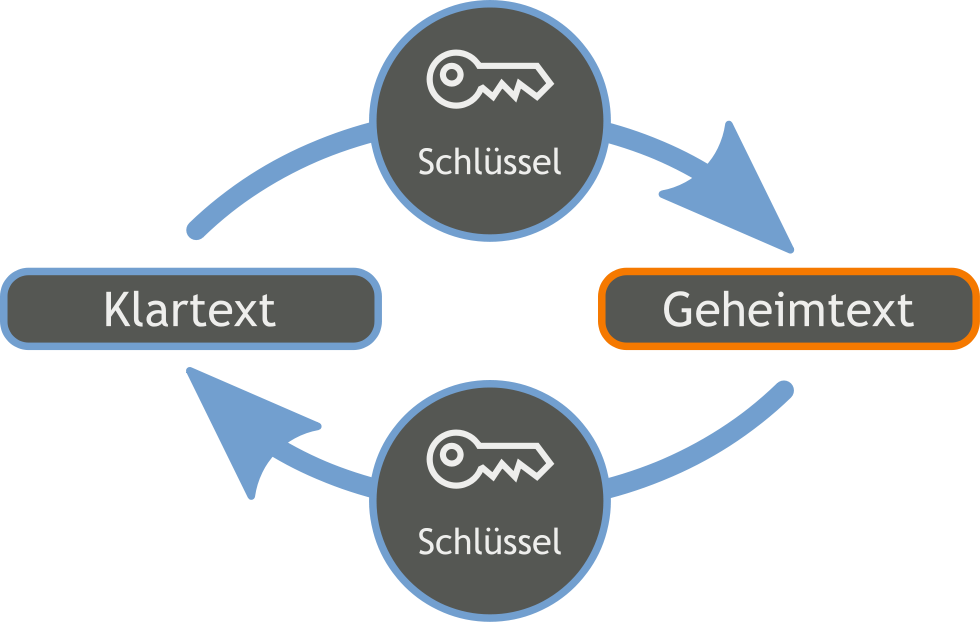
\includegraphics[scale=0.4]{images/sym_crypt}%
\end{minipage}}

\protect\caption{Symmetrische Kryptographie}
\end{figure}



\subsection*{Symmetrische Schlüssel \label{sub:Symmetrische-Schl=0000FCssel}}

Es handelt sich um einen geheimen Schlüssel, der beim AES-Algorithmus
(Symmetrische Verschlüsselungsverfahren) eingesetzt wird, um Chiffrierung
und Dechiffrierung durchzuführen. Da die symmetrischen Schlüssel sowohl
zur Chiffrierung als auch zur Dechiffrierung eingesetzt werden, sind
sie als kritische Informationen zu sehen. 


\subsection*{Dateischlüssel}

Ein Dateischlüssel ist ein symmetrischer Schlüssel, der eingesetzt
wird, um Dateien zu chiffrieren bzw. zu dechiffrieren. In dieser Arbeit
entspricht der Dateischlüssel den Gruppenschlüssel, kurz SGK (Secret
Group Key). 


\subsection*{Passwort und Passphrase }

Duden \cite{duden:passwort} definiert das Passwort bzw. Passphrase
wie folgt : 
\begin{quote}
,,nur Eingeweihten bekannte, aus Buchstaben, Ziffern oder Sonderzeichen
bestehende Zeichenfolge, die den Gebrauch einer Sache, den Zugang
zu ihr ermöglicht und sie gegen den Missbrauch durch Außenstehende
schützen soll.``
\end{quote}
Der Begriff ,,Passwort`` wird in der Dokumentation benutzt im Zusammenhang
mit Benutzeranmeldeinformationen, und wird in einer modifizierten
Form im RemoteServer gespeichert. Hingegen wird Passphrase außerhalb
des LocalServers nie persistent gehalten. Das Passphrase wird angewandt,
um den Benutzer-Masterkey zu verschlüsseln.


\subsection*{Digitale Signature \label{sub:Digitale-Signature}}

Eine digitale Signatur, auch digitales Signaturverfahren, ist ein
asymmetrisches Kryptosystem, bei dem ein Sender mit Hilfe eines geheimen
Signaturschlüssels (dem privaten Schlüssel) zu einer digitalen Nachricht
einen Wert berechnet, der ebenfalls digitale Signatur benannt wird.
Dieser Wert ermöglicht es jedem, mit Hilfe des öffentlichen Verifikationsschlüssels
(dem öffentlichen Schlüssel) die nicht bestreitbare Urheberschaft
und Integrität der Nachricht zu prüfen. Um eine mit einem Signaturschlüssel
erstellte Signatur einer Person zuordnen zu können, muss der zugehörige
Verifikationsschlüssel dieser Person zweifelsfrei zugeordnet sein.


\section*{Hybride Verschlüsselung }

Hybride Verschlüsselung ist eine Kombination aus asymmetrischer Verschlüsselung
und symmetrischer Verschlüsselung. Dabei wählt der Sender einen zufälligen
symmetrischen Schlüssel, der Session-Key genannt wird. Mit diesem
Session-Key werden die zu schützenden Daten symmetrisch verschlüsselt.
Anschließend wird der Session-Key asymmetrisch mit dem öffentlichen
Schlüssel des Empfängers verschlüsselt. Dieses Vorgehen löst das Schlüsselverteilungsproblem
und behält dabei den Geschwindigkeitsvorteil der symmetrischen Verschlüsselung.

\begin{table}
\begin{tabular}{|c|c|c|}
\hline 
 & asymmetrische Verschlüsselung & symmetrische Verschlüsselung\tabularnewline
\hline 
\hline 
Effizienz & langsam & schnell\tabularnewline
\hline 
Schlüsellaustausch & elegant & problematisch\tabularnewline
\hline 
\end{tabular}

\protect\caption{Vergleich asymmetrische/symmetrische Verschlüsselugn}
\end{table}


Wie die Abbildung oben zeigt, sind symmetrische Verschlüsselungsverfahren
auch bei großen Datenmengen sehr schnell, asymmetrische dagegen sind
sehr langsam, und deshalb nur für kleine Datenmengen (wie etwa für
Schlüssel) geeignet. \\
Bei der Schlüsselverteilung hat das symmetrische Verschlüsselungsverfahren
den Nachteil, dass sich die Kommunikationspartner vor der Übermittlung
der Nachricht auf einen geheimen Schlüssel einigen müssen. Dazu muss
ein sicherer Kommunikationskanal benutzt werden, wie zum Beispiel
ein Kurier. Asymmetrische Verschlüsselungsverfahren dagegen lösen
das Problem sehr elegant, weil zum Verschlüsseln nur der öffentliche
Schlüssel gebraucht wird. Zur Übermittlung dieses Schlüssels reicht
ein authentifizierter Kanal aus. \\
Hybride Verschlüsselungsverfahren kombinieren die beiden Verfahren
(asymmetrisch und symmetrisch) so, dass deren Vorteile erhalten bleiben: 
\begin{itemize}
\item Hybride Verschlüsselungsverfahren sind sehr schnell und eignen sich
für große Datenmengen, weil die Daten mit dem symmetrischen Verfahren
verschlüsselt werden und das asymmetrische Verfahren nur für den Sitzungsschlüssel
verwendet wird.
\item Es muss vor dem Senden der Nachricht kein geheimer Schlüssel ausgetauscht
werden. Die Kenntnis des öffentlichen Schlüssels des Empfängers reicht,
um zu verschlüsseln.
\end{itemize}

\section*{Public Key Infrastructur (PKI)}

Public Key Infrastructur ist ein System, das digitale Zertifikate
ausstellen, verteilen und prüfen kann. Die innerhalb einer PKI ausgestellten
Zertifikate werden zur Absicherung Rechner-gestützter Kommunikation
verwendet. \\
Basis für Public Key Infrastructur sind das asymmetrische Kryptosystem
und die hybride Verschlüsselung. Mit Hilfe des asymmetrischen Kryptosystems
werden die Daten digital signiert und verschlüsselt. 


\section{Email }

Der Austausch von elektronischen Daten per Email ist weit verbreitet.
Email-Dienste werden von eigenen Unternehmen oder auch von Internet-Dienstleistern
angeboten. Die Versendung von Emails über das Internet ist zunächst
unverschlüsselt. Somit sind die Inhalte relativ einfach auch für Dritte
lesbar. \\
Die Identitäten der Kommunikationspartner werden i. Allg. mit den
Email-Adressen gleichgesetzt. Eine weitergehende Prüfung findet nicht
statt. Dadurch aber wird der Identitätsdiebstahl erleichtert, das
heißt die Vortäuschung einer fremden Identität (Email-Adresse). Obwohl
in der meisten Email-Clients eine Funktion vorgesehen ist, um das
Risiko des Identitätstäuschung zu umgehen, geschieht die Email-Adressenüberprüfung
nicht automatisch. Dies bleibt dem Benutzer überlassen. \\
Ein Austausch über Firmengrenzen hinweg ist problemlos möglich. Problematisch
ist aber der Austausch von kritischen Informationen. 

Eine auf dem ersten Blick triviale Lösung, was das Austauschen von
sensiblen elektronischen Daten angeht, besteht darin, die Daten zu
verschlüsseln und diese per Email an den Kommunikationspartner zu
senden. Diese Lösung ist nur möglich, sofern sich die Teilnehmer (Sender
und Empfänger) mit Kryptographie bzw. Kryptographiesoftware auskennen.
\\
Überhaupt stellen sich dieser Lösung etliche Hürden in den Weg: 
\begin{itemize}
\item Wie gerade erwähnt, setzt diese Lösung voraus, dass sich die Kommunikationspartner
mit der Kryptographie bzw. Kryptographiesoftware auskennen. 
\item Zusätzliche Softwareinstallationen sind zwingend erforderlich. 
\item Der Schlüsselaustausch ist problematisch, und zwar insofern, als der
Dechiffrierschlüssel an den Kommunikationspartner übermittelt werden
muss.
\item Dazu kommt noch die Infrastrukturproblematik: Schlüsselmanagement,
Sicherheit der Schlüssel, Software-Installation etc. ... 
\end{itemize}

\section{Web-upload\label{sec:Web-upload}}

Das Speichern von Dokumenten auf einem Internet-Server ist weit verbreitet
und weltweit von jedem Browser aus möglich. Eine Installation zusätzlicher
Software, oder gar die Öffnung zusätzlicher Ports der Unternehmens-Firewall
ist nicht erforderlich. Die Benutzer-Authentifizierung erfolgt i.d.R.
per Login/Password. Daten können im Internet mittels des http-Protokolls
verschlüsselt übertragen werden. Fälschlicherweise wird angenommen,
dass die übertragenen Dokumente dann auch beim Empfänger „sicher“
gespeichert sind. Jedoch werden lediglich die Dokumente auf dem Weg
zum Server mit SSL verschlüsselt. Danach liegen sie zunächst unverschlüsselt
vor. So werden von einem Server verschlüsselt übertragene Dokumente
vom Browser entschlüsselt und im Klartext auf dem lokalen PC gespeichert.
Ebenso werden Dokumente, die vom Browser für die Übertragung verschlüsselt
werde, vom Server entschlüsselt und liegen dann am Server unverschlüsselt
vor. Somit ergeben sich dieselbe Problematik und derselbe Lösungsansatz
wie bei Datei-Servern. In Folge dessen sollten Dokumente, die per
Browser auf einen Datei-Server geladen werden, vom Client-PC verschlüsselt
wer- den. Die Dokumente müssen also vor dem Upload verschlüsselt worden
sein, oder aber der Browser führt die Verschlüsselung durch. Eine
Vorab-Verschlüsselung der Dateien hat den Nachteil, dass das Dokumenten-
und Schlüssel-Management vom Anwender eigenverantwortlich durchgeführt
werden muss. Dies ist den Anwendern i. Allg. zu aufwendig. Folglich
sollte die Verschlüsselung durch den Browser quasi automatisch erfolgen.
Dies wird aktuell nur sehr selten durchgeführt, da die Verschlüsselungs-Softwares
auch vom Web-Server geladen werden müssen. Und es kann nicht garantiert
werden, dass die geladene Software nicht Eindringlingen unbeabsichtigten
Zugriff ermöglicht. In Folge dessen werden Dokumente SSL-verschlüsselt
zum Server gesendet. Die dort empfangenen, unverschlüsselten Dokumente
werden sofort verschlüsselt und als Datei abgelegt.\\
Hier bestehen jedoch folgende Probleme: 
\begin{itemize}
\item Wie kommen die notwendigen Schlüssel zum Server? 
\item Ein Eindringling auf dem Server kann die Klartext-Datei und/oder die
Schlüssel mitlesen
\end{itemize}
Zusammenfassung: Ein Ansatz für ein sicheres web-upload ist bisher
nicht bekannt.


\section{File Transfer Protocol (FTP) }

Das File Transfer Protocol (Dateiübertragungsprotokoll) ist ein in
RFC 959 \cite{RFC959} spezifiziertes zustandbehaftetes Netzwerkprotokoll
zur Übertragung von Dateien. FTP läuft in der Anwendungsschichtmodell.
Es wird benutzt um Dateien von Server zu Client herunterzuladen bzw.
von Client zum Server hoch zu laden. \\


Eine wesentliche vorteilhafte Eigenschaft von FTP ist, dass die meisten
Betriebssysteme (Unix basierende zum Beispiel) werden mit FTP-Client-und-Server
vorinstalliert. Dadurch ist kein zusätzliche Softwareinstallation
nötig. \\
Es existieren zahlreiche robuste FTP-Clients von Terminal-Client (mit
Linux vorinstalliert) bis GUI-Client ( Filezilla ), welche die auch
als Mozilla-Firefox oder Chrome Addons benutzt werden können.\\
Mit dem Ziel, bessere Sicherheit zu gewährleisten, wurde SFTP (SSH
Transfer Protocol) implementiert. SFTP ist eine alternative zum FTP.
SFTP benutzt eine sichere Kanal mit Hilfe von SSH für Dateitransfer.


\section{Cloud-Service }

Cloud-Service hat sich in den letzten fünf Jahren wesentlich verbreitet.
Und war auf einer guten Weg bis zum NSA-Affäre sich als Standard einzusetzen.
Heute auch trotz die Spionageskandale, wird Cloud-Service bei viele
Endbenutzer sehr beliebt. Gerade bei der Bereitstellung von sensiblen
Dokumenten über die Cloud ist es unumgänglich, auf Sicherheit und
Schutz vor fremdem Eingriff zu achten. Doch oft möchte man, einige
Dateien mit einem Geschäftpartner oder Kollegen austauschen und achtet
wenig auf Sicherheit. Beliebte Cloud-Lösungen aus dem Privatbereich
wie Dropbox werden hierbei gerne verwendet. Die Richtlinien solcher
Cloud-Speicher entsprechen nicht dem deutschen Datenschutzrecht. Einer
der eventuelle gravierende Problem ist es dass die Daten unverschlüsselt
abgespeichert werden, Anders ausgedruckt, ein Dritter benötigt nur
die Benutzer-Credentials, um das Dokument unverschlüsselt runter zu
laden. Möchte man sein Dokument verschlüsselt hoch laden, muss man
sich selber darum kümmert, dadurch entstehen die gleiche Problematiken
wie beim Webupload\ref{sec:Web-upload} 


\section{PGP }

\begin{figure}
\fbox{\begin{minipage}[t]{1\columnwidth}%
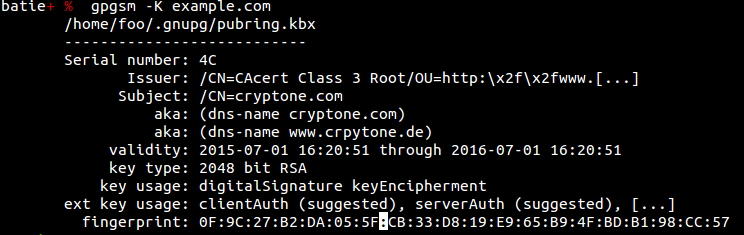
\includegraphics[scale=0.56]{images/pgp_screenshot}%
\end{minipage}}

\protect\caption{examplarische zertifikat }
\end{figure}


PGP {[}Zim95{]} {[}ASZ96{]} {[}Sta95{]} ist eine Daten-Ver- und Entschlüsselung
Computerprogramm, das kryptographische Privatsphäre und Authentifizierung
für die Datenkommunikation zur Verfügung stellt. PGP wird oft zum
Signieren und zur Ver-und Entschlüsselung von Texten, E-Mails, Dateien
und Verzeichnisse verwendet, um die Sicherheit der E-Mail-Kommunikation
zu erhöhen. Es wurde von Phil Zimmermann im Jahr 1991 entwickelt.\\
Im PGP-System wird für einen Benutzer ein Schlüsselpaar (öffentlicher
Schlüssel und privater Schlüssel) erzeugt. Dieses Schlüsselpaar ist
mit einer eindeutigen ID verbunden, die normalerweise ein Name oder
eine Email-Adresse ist. Die Schlüssel werden in einem Schlüsselbund
Datensatz gespeichert.Der Eintrag eines öffentli- chen Schlüssels
im Schlüsselbund besteht aus einer ID, dem öffentlichen Schlüssel
selbst und einem Zeitstempel, der auf das Erstellungsdatum des Schlüsselpaars
referenziert. Öffentliche Schlüssel werden auf einem öffentlichen
Schlüsselring gespeichert, wohingegen private Schlüssel auf einem
privaten Schlüsselring gespeichert werden. Jeder Benutzer muss einen
öffentlichen und privaten Schlüsselring speichern und verwalten{[}AR95{]}{[}JF96{]}.
Wenn Benutzer A eine gute Kopie des öffentlichen Schlüssels von Benutzer
B besitzt, z.B. eine Kopie, deren er von der Integrität und Authentizität
(keine Verfälschung etc.) überzeugt ist, dann kann A diese Kopie unterschreiben
und an Benutzer C weitergeben. A wirkt somit als eine Mittelsperson
von B zu C. Der von A signierte Schlüssel wird als Schlüssel Zertifikat
bezeichnet. Jeder Benutzer muss im PGP-System erklären, welchen Personen
er oder sie als Mittelsperson vertraut und muss den öffentlichen Schlüssel
der Mittelsperson mit seinem eigenen privaten Schlüssel signieren.
Außerdem muss der Benutzer die verschiedenen Vertrauensgrade angeben,
welche er zu seinen Mittelsperson hat. Eine Vertrauensbeziehung zu
einer Person kann in Graden als unbekannt, nicht vertrauenswürdig,
geringfügig vertrauenswürdig oder vollständig eingestuft, also klassifiziert
werden. Jeder Benutzer speichert seine vertrauten Informationen oder
Zertifikaten auf seinem in seinem PGP Konto. Abhängig vom Vertrauensgrad
zu einer Mittelsperson ist dem entsprechenden Zertifikat im Schlüsselbund
einen Gültigkeitsgrad zugewiesen. Er kann den Schlüssel in diesem
Zertifikat nur dann verwenden, wenn der Gültigkeitsgrad hoch genug
ist. Zum Beispiel kann ein skeptischer Anwender zwei vollständige
Unterschriften für einen öffentlichen Schlüssel einfordern, um ihn
als gültig anzusehen, wohingegen ein wenig skeptischer Benutzer, nur
eine vollständig vertrauenswürdige Signatur oder zwei geringfügig
vertrauenswürdige Signaturen verlangen könnte. Es ist wichtig zu beachten,
dass Schlüsselringe und Vertrauensgrade es ermöglichen, jedem Benutzer
seine eigene Vertrauenspolitik zu gestalten. Diese enge Vorstellung
von Politik ist in PGP angebracht, denn es wurde speziell entworfen,
um sichere E-Mails für den Einzelnen bereitzustellen. Die Unterschrift
von A auf öffentlichen Schlüssel von B nicht so interpretiert werden
sollte, dass A der persönliche Integrität von B vertraut. Die richtige
Interpretation ist eher, dass A glaubt, dass die Bindung der Identität
von B zum Schlüssel richtig ist. Darüber hinaus ist es wichtig zu
beachten, dass das Vertrauen nicht transitiv ist. Die Tatsache, dass
A dem B vollständig als Mittelsperson vertraut und dass B vollständig
C vertraut, bedeutet nicht automatisch, dass A mit dem gleichen Grad
C vertraut. Da PGP in der Popularität gewachsen ist, ist ein dezentrales
\textquotedbl{}Web of Trust`` entstanden. Jedes Individuum ist verantwortlich
für den Erwerb der öffentlichen Schlüssel, die er braucht, und für
die Zuordnung des Vertrauensgrads zu den Mittelpersonen, von denen
er sie bekommt. Ähnlich muss jedes Individuum sein eigenes Schlüssel-
paar erstellen und seinen öffentlichen Schlüssel verbreiten. Sein
Ansatz lehnt folglich die Benutzung der offiziellen Zertifizierungsstellen
ab, welche die öffentlichen Schlüssel eines Individuums unterschreiben.
Damit handelt eine einzelne Person als \textquotedbl{}Vertrauensserver\textquotedbl{}für
die Benutzer von diesen Schlüsseln. Ein Vorteil von PGP ist, dass
jeder Benutzer denjenigen vertrauen (öffentlichen Schlüssel signieren)
kann, denen er will. Außerdem bietet PGP die Möglichkeit, Gruppen
zu erzeugen und in dieser Gruppe verschlüsselte Nachricht oder Dateien
zwischen den Mitgliedern auszutauschen. Der erste Nachteil von PGP
ist, dass die Software auf dem lokalen Rechner installiert werden
muss und dort alle Schlüssel gespeichert werden. Wie soll der Benutzer
dann seinen Schlüssel in einem anderen System oder in einer anderen
IT-Infrastruktur benutzen. Die Schlüssel können zwar exportiert und
importiert werden, jedoch führt dies zu einem erhöhten Aufwand. Ferner
stellt sich die Frage, wie der Benutzer es einem Vertrauten ermöglicht,
seine Schlüssel zu verwenden? Außerdem stößt die lokale Installation
der Software auf bestimmte Anforderungen.


\section{X.509}

Der X.509 {[}Ada99{]} {[}CDH + 05{]} Authentifizierungsframework versucht,
den gleichen Teil des Vertrauen-Management Problems wie PGP zu lösen,
nämlich die Notwendigkeit, eine entsprechend zuverlässige vertrauenswürdige
Kopie des öffentlichen Schlüssels einer Person zu finden, mit der
man kommunizieren will. Wie in PGP, sind X.509-Zertifikate unterzeichnete
Datensätze, welche die Benutzer ID mit ihrem kryptographischen Schlüssel
assoziieren. X.509-Zertifikate enthalten weitere Informationen über
PGP-Zertifikate, wie zum Beispiel den Namen des verwendeten Signatur-Verfahrens,
um sie zu erstellen und das Zeitintervall, in dem sie gültig sind.\\
Aber ihr Hauptziel ist einfach die Bindung zwischen Benutzern zu ihren
Schlüsseln zu schaffen. Jedoch unterscheidet sich X.509 scharf von
PGP im Grad der Zentralisierung der Informationen. In PGP kann jeder
öffentliche Schlüssel signieren und damit als Mittelsperson handeln.
Der X.509 Framework fordert dagegen, dass jeder Benutzer seine Zertifikate
von einer offiziellen Zertifizierungsstelle (CA) erhalten muss. Wenn
Benutzer A ein Schlüsselpaar (öffentlicher Schlüssel , privater Schlüssel)
erstellt, muss er es und die Rest der erforderlichen Informationen
von einem oder mehreren CAS zertifizieren lassen und die erhaltenen
Zertifikate in einem offiziellen Verzeichnisdienst registrieren. Wenn
A später mit B sicher kommunizieren will, erhält er ein Zertifikat
von B aus dem Verzeichnis-Server. Wenn A und B von der gleichen CA
zertifiziert wurden, kann nur der Verzeichnisserver B’s Zertifikat
zu A senden. A kann dann die Gültigkeit dieser Zertifikat mit dem
öffentlichen Schlüssel dieser gemeinsamen CA prüfen kann. Wenn A und
B nicht unmittelbar durch eine gemeinsame CA zertifiziert werden,
dann die Verzeichnisdienst müssen einen Zertifizierung-Pfad von A
nach B erstellen. Um diesen Pfad zu verwenden, muss A den öffentlichen
Schlüssel von der erste Zertifizierungsstelle in dem Pfad kennen.
Somit beruht X.509 Framework auf der Annahme, dass CAs zu einem globalen
Zertifizierungsstellen Baum-organisiert sind und dass alle Benutzer,
die von CAs mit einem gemeinsamen Vorfahren in diesem globalen Baum
unterzeichnet wurden{[}DWC03{]} {[}HPFS02{]} {[}CD03{]}.\\
Das Problem ist, dass der Benutzer nicht eine autonome Identität einer
weiteren Person prüfen kann, denn er ist vom öffentlichen Schlüssel
seiner CA abhängig. Außerdem vertraut er automatisch alle Personen,
denen die Öffentlichen Schlüssel durch die selbe Zertifizierungsstelle
signiert wurden oder durch einer anderen vertrauten Zertifizierungsstelle.
Dies stößt gegen einige Anforderungen, die fordern, dass die Benutzer
nur gewünschte Personen vertrauen müssen. Darüber hinaus hat die NSA
Affären bewiesen, dass Zertifizierungsstelle verfälschte Zertifikate
erstellen können und somit werden verfälschte Identitäten freigegeben.


\section{SPKI / SDSI}

SDSI {[}EFL + 99{]}{[}RL96{]} {[}ST00{]} wurde von Ronald Nieten und
Butler Lampson konzipiert. Seine Entwicklung wurde durch die Komplexität
der herkömmlichen Public-Key Infrastrukturen speziell die Abhängigkeit
auf den globalen Namensraum motiviert. SDSI ist eine Public Key-Infrastruktur
mit lokalen Namensraum. Dies macht es zu einem dezentralen Sicherheitssystem.
SPKI wurde von Carl Ellison entwickelt und Andere. Es ist ein einfaches
Autorisierungs-System. Hier wird der öffentliche Schlüssel nicht dazu
genutzt, die Identität des Schlüsselbesitzers zu prüfen, sondern direkt
seine Berechtigung zu bestimmten Diensten zu definieren. Die Vereinigung
der beiden Projekte führt zum SPKI / SDSI, ein System zur Autorisierung
und Authentifizierung. das SDSI lokalen Namensräume mit SPKI Autorisierung
Systems kombiniert. SPKI / SDSI ist eine vollständig verteilte Lösung.
Jeder Benutzer wird eine Zertifizierungsstelle und ist für die Verwaltung
von Zertifikaten selbst zuständig. In SPKI / SDSI werden die Benutzer
durch einen öffentlichen Schlüssel identifiziert und der öffentliche
Schlüssel ist einem lokalen Benutzernamen Raum zugeordnet. Dieser
Verein ist gültig lokal, das heißt, die zugehörigen Namen sind nicht
global eindeutig. SPKI / SDSI erlaubt die Definition von Gruppen von
Benutzern. Hier werden die öffentlichen Schlüssel der Mitglieder einer
Gruppe des gleichen Namens zuge- ordnet. In SPKI / SDSI, gibt es zwei
Arten von Zertifikaten: Namenszertifikate und Berechtigungszertifikate.
Das Namenszertifikat bescheinigt, dass ein Name in einem Namensraum
eines Emittent gültig ist. Das Berechtigungszertifikat gewährt den
Res- sourcenzugriff eines Benutzers. Namenszertifikate bestehen aus
vier Bereichen zusammen:Issuer(Emittenten), Iden- tifier( Identifizierter),
Subject (Subjekt) und validity specification (Gültigkeit Spezi- fikation).
Der Issuer ist derjenige, der das Zertifikat unterzeichnet. Der Identifizierter
ist ein Byte, Zeichenkette, die einen Namen repräsentiert. Das Subject
kann ein Name sein, oder ein öffentlicher Schlüssel. Wenn das Subject
ein Name ist, ist es in lokalen Namenraum und der damit verbundene
öffentliche Schlüssel kann wieder- hergestellt werden. Schließlich
Gültigkeit Spezifikation ist eine Gültigkeitsbedin- gung des Zertifikats,
es könnte ein Gültigkeitsdatum oder eine Zugriffssteuerungs- liste
(ACL) sein. Berechtigungs Zertifikat besteht aus fünf Bereichen: Issuer(Emittenten),
subject(Subjekt), Delegation, Tag, und ihrer Gültigkeit Spezifikation.
Issuer und subject haben die gleiche Funktion wie oben geschrieben.
Jedoch kann das Subject eine Gruppe von Nutzer sein. Das Feld Delegation
zeigt an, dass das Zertifikat auch zu anderen Sub- jekten übertragen
werden könnte. Tag gibt an, welche Berechtigungen empfangen wurden.
Wie im Fall der Namenszertifikate ist Gültigkeit Spezifikation eine
Gültig- keitsbedingung des Zertifikats {[}CEE + 01{]} {[}HM99{]}.
Hier wird ein kurzes Beispielszenario genannt: Der Dateisystemressource
Besitzer erzeugt zwei Berechtigungszertifikate. Ein Zertifikat ist
mit der erteilten Zulassung: lesen, schreiben und nicht Delegation
(RW: ND) zu D1 gegeben. Ein anderes Zerti- fikat ist an D2 mit Genehmigung
: lesen und Delegation (R: D) gegeben. In der glei- chen Figur erzeugt
D2 eine neue Zertifikat für D3 mit Leserechten, aber Delegation nicht
erlaubt (R: ND). Wenn D3 auf das Dateisystem zugreifen muss, präsentiert
er die Delegation Kette (D2 R: D - -> D3 R: ND) zu dem System.\\
Der Besitzer einer Datei will zum Beispiel den Zugriff auf die Dateien
an viel Benutzer freigeben, dafür muss er jeweils ein Zertifikat mit
den gewünschten Berechtigungen unterschreiben.


\chapter{Anforderungen\label{chap:Anforderungen}}

Bei der Anförderungsanalyse unterscheidet man zwischen funktionalen
und nichtfunktionalen Anforderungen. Während funktionale Anforderungen
den gewünschte Verhalten und die Funktionalität vorgeben, beschreiben
nicht- funktionale Anforderungen Rahmenbedingungen wie Performance
oder Zuverlässigkeit.


\section{funktionale Anforderungen}

Funktionale Anforderungen

\begin{figure}
\fbox{\begin{minipage}[t]{1\columnwidth}%
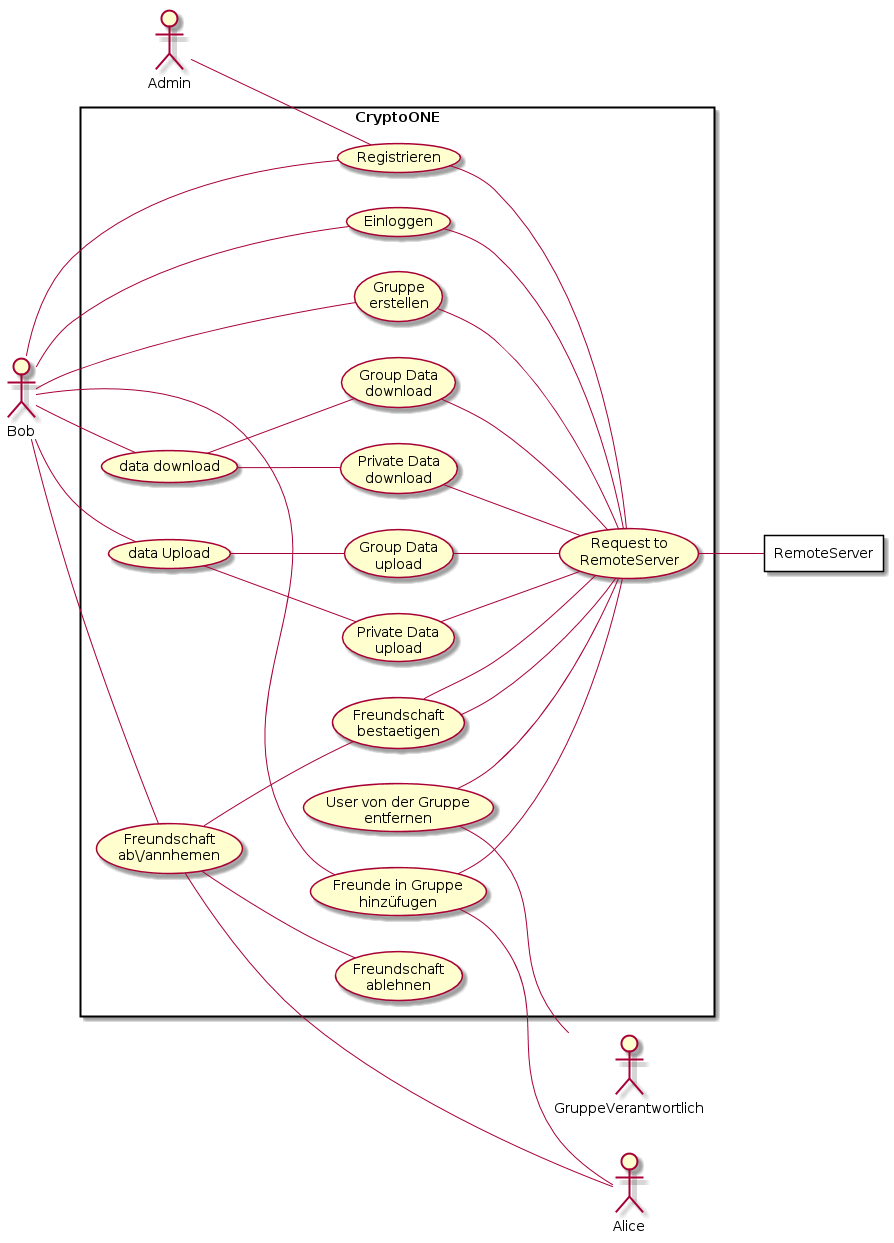
\includegraphics[clip,angle=360,origin=c,scale=0.45]{images/src/pu/usecase/functionaleAnforderungen}%
\end{minipage}}

\protect\caption{Funktionale Anforderungen Überblick}


\end{figure}



\subsubsection{Administrator Rolle}
\begin{itemize}
\item Der Administrator muss in der Lage sein, neue Benutzer im System hinzu
zu fügen und zu entfernen. 
\item Der Administrator darf nicht in der Lage sein, Benutzer kritische
Informationen zu modifizieren oder zu lesen.
\end{itemize}

\subsubsection{Benutzer role}
\begin{itemize}
\item Der Benutzer kann eine Vertrauensbeziehung zu anderen Benutzern herstellen
und sie wieder zurückziehen. 
\item Der Benutzer kann eine Gruppe bilden und wieder auflösen.
\item Der Benutzer kann einer Gruppe vertraute Benutzer (Friends) hinzufügen.
\item Der Benutzer kann den Zugriff auf seine Dateischlüssel an alle Mitglieder
einer Gruppe freigeben und diese Freigabe auch wieder zurückziehen.
\end{itemize}

\subsubsection{Registrierung und login}
\begin{itemize}
\item Bei der Registrierung bzw. beim Login Phase dürfen kein Password oder
keine Passphrase sowie Daten, die in irgendeiner Art mit dem Password
bzw. mit der Passphrase korrespondieren, ins Netz gehen.
\end{itemize}

\subsubsection{Server-Client Kommunikation }
\begin{itemize}
\item Die Verbindung zwischen ~LocalServer~ und ~RemoteServer~ sollte
Zustand-los sein. 
\item es darf keine SSL Verbindung zum Einsatz kommen. 
\item Server und Client müssen in der Lage sein sich gegenseitig zu authentifizieren.
\end{itemize}

\section{Nicht-funktionale Anforderungen }

Nicht-funktionale Anforderungen sind wie folgt in ISO/IEC 9126\cite{ISO/IEC9126}
erklärt: 

TODO


\subsection{Allgemeine nichtfunktionale Anforderungen}
\begin{itemize}
\item Kein Einsatz von HTTPS 
\item RemoteServer darf keine Verschlüsselung bzw. Entschlüsselung durchführen 
\item LocalServer soll von ein USB-Stick gestartet werden, und soll auch
von dort aus im Hintergrund laufen. 
\item Benutzerinteraktion erfolgt durch ein Browser so, dass keine zusätzliche
Software-Installation erforderlich ist.
\end{itemize}

\subsection{Wartbarkeit und Erweiterbarkeit}

Die resultierende Software dieser Arbeit, soll in Zukunft gewartet,
erweitert und verändert werden. Neu Features sind schon festgelegt
( sollen aber in der jetzige Version nicht implementiert werden )


\subsection{Portierbarkeit und Plattform-Unabhängigkeit}

Defakto ist der LocalServer portierbar, LocalServer läuft auf USB-Stick
. Localserver soll auch plattformsunabhängig sein. Was RemoteServer
angeht soll auch plattformunabhängig sein. Alle Einstellungen des
Remoteserver müssen sich durch externe Konfigurationsdateien durchführen
lassen.


\subsection{Daten-und Serverintegrität}

Der Benutzer soll in der Lage sein die Integrität von RemoteServer
zu prüfen und der auf der letzer abgespeicherte Daten.


\chapter{Konzept}


\section{Allgemein Architektur}

Das System Architektur wurde als eine Server-Client Anwendung entworfen,
LocalServer und RemoteServer, wobei der LocalServer eine Überbrückungsrolle
zwischen den Frontend (Webbrowser Javascriptapplication) und RemoteServer
spielt, LocalServer ist vergleichbar mit ein Proxy. Alle Chiffrierung-bzw-Dechiffrierungoperationen
geschehen. 

\begin{figure}
\fbox{\begin{minipage}[t]{1\columnwidth}%
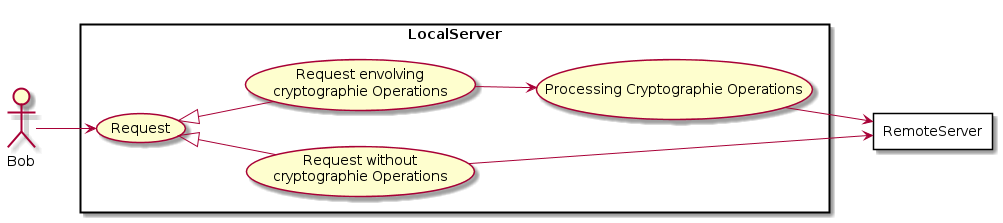
\includegraphics[clip,scale=0.4]{images/src/pu/usecase/generalUsecase}%
\end{minipage}}

\protect\caption{Allg. Architektur}


\end{figure}



\section{Authentifizierung}

Authenfizierung spielt systemweit eine bedeutende Rolle. Dabei passieren
alle notwendige Prüfung von {[}LocalServer{]}, {[}RemoteServer{]},
{[}RemoteServer{]} integrität und natürlich Verifizierung von Benutzer.
Es durfte systemweit keine Einsatzt von Zertifikat/SSL-Verbindung
oder Aufbau eine zustandbehaft Verbindung kommen, spricht die Kommunikationskanal
ist unsicher. Um Benutzercredentials von {[}LocalServer{]} auf {[}RemoteServer{]}
zu übermitteln unter Anhaltung von Spezifikation, wurde SRP \cite{RFC2945}
(Secure Remote Password) eingesetzt.\\
Beim Einsatz von SRP-Secure Remote Password Protocol lasst sich auch
einfach der gegenseitige Aunthenfizierung von {[}LokalServer{]} und
{[}Remote- Server{]} realisieren, diese geschehet auch beim Authentifizierungsphase.\\
SRP Protokoll ist ein Authentifizierung protokoll, dabei können manche
per-Sitzung zufällige generierte Werte als Sitzungschlüssel verwendet
werden (B). Das bestehende Problem beim Einsatzt von dauerhafte Passwort
wird durch SRP minimisiert, indem keine Passwort-korrespondierte (
Hash, verschlüsselte Passwort .... ) gepeichert wird, sondern ein
,,Verifier``. Gewinn ein Eingreiffer die auf den Datenbank gepeichert
,,Verifier`` , dann kann der nicht daraus die Benutzerpasswort wiederrechnen.
Ein gestohlener Verifier ist ebenso nicht ausreichend zür Anmeldung,
Weil das Passwort immer noch benötigt wird.\\
Zur erfolgreiche Authentifizierung wird kein sensible Information
ausgetausch ,,Sniffing-Attack`` ist dann dabei hilflos. 

\begin{figure}
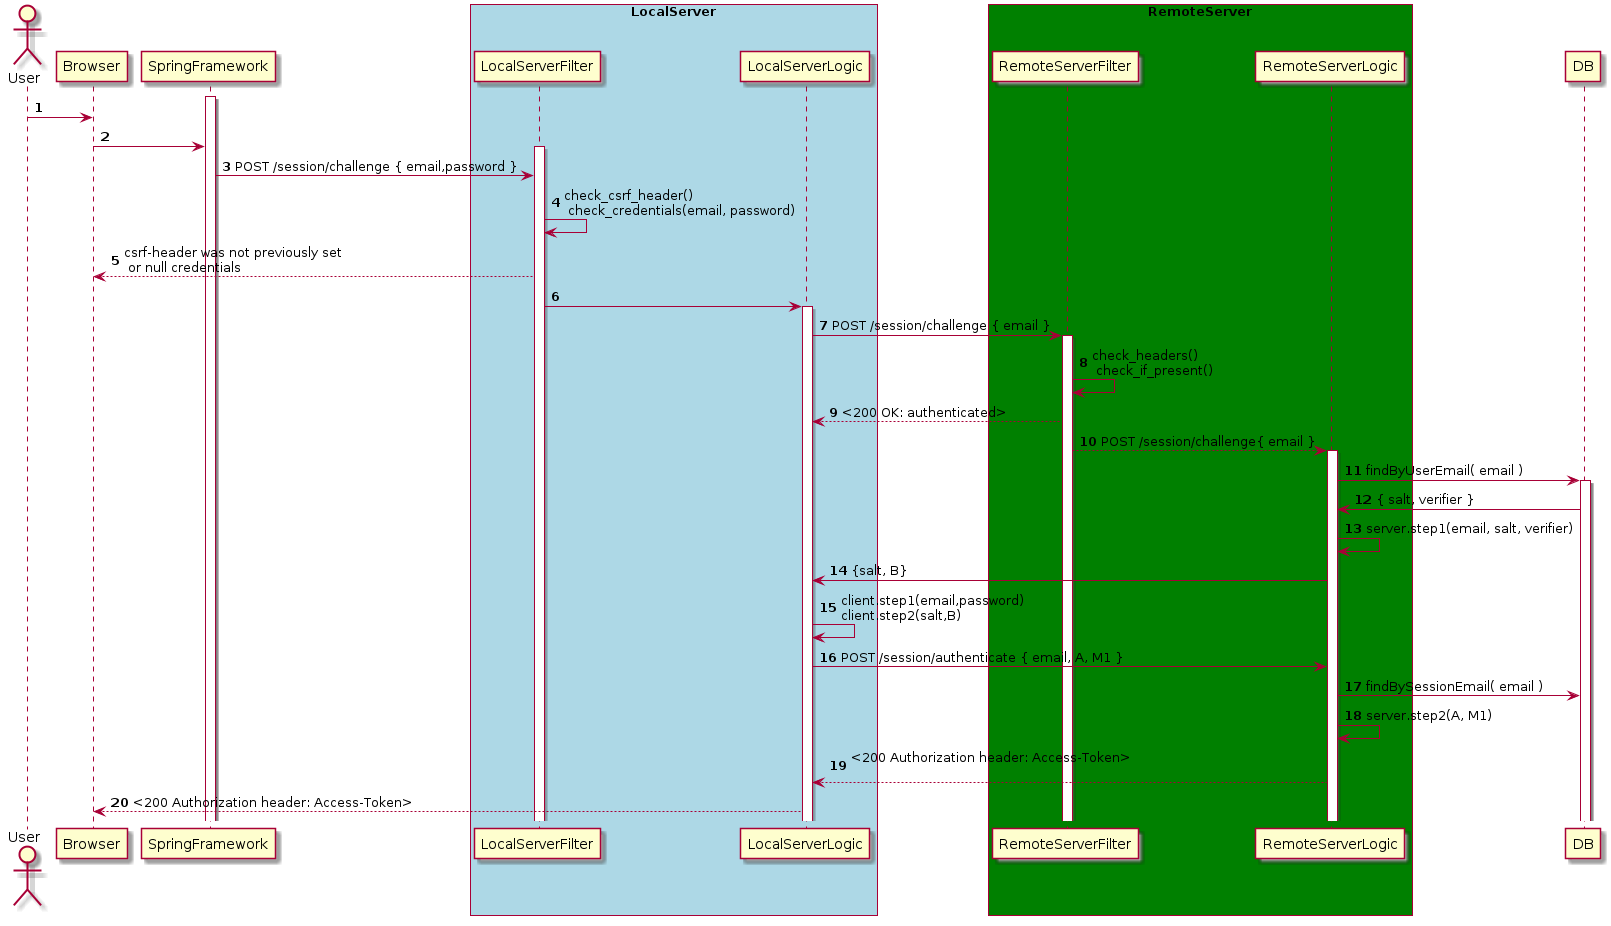
\includegraphics[angle=90,scale=0.4]{images/src/pu/sequence/localServer}

\protect\caption{Authenticationsablauf}


\end{figure}



\section{Kritische Daten Integrität}


\section{Schlüsselaustausch}

Dokumentenschlüssel stehen nicht direkt in Verbindung mit Benutzer
sondern mit der Gruppe. Wenn eine Gruppe kreiert wird, wird eine Gruppenschlüssel
erzeugt. Dieser Schlüssel wird mit öffentliche Schlüssel der Gruppe-verantwortlich
(GV) verschlüsselt. Jeder Benutzer der in der Gruppe eingeladen wird,
bekommt dann eine Kopie der Gruppenschlüssel. Falls der zuvor eingeladenen
Benutzer wieder durch der Gruppe-verantwortlich aus der Gruppe gelöscht
wird, dann wird auch seiner Kopie der Gruppenschlüssel gelöscht sowie
seine Verbindung zur Gruppe. 


\section{Server Integrität \label{sec:local_server_public_key}}

Beim eine sicherheitrelevante Anwendung ist es wichtig an jeder Anwendungfälle
an der Integrität der Softwareteile zu prüfen, sowie auch von exportierte
Daten. Neben der Authentifizierung von Benutzer an sich, muss sich
LocalServer an RemoteServer authentifizieren sowie RemoteServer an
LocalServer. \\
RemoteServerintegritätsprüfung gescheht beim der Allererste Loginversuch,
sowie beim jeder weiteren Request von LocalServer zu RemoteServer.\\
Dank SRP6-A Protokoll können LocalServer und RemoteServe sich gegenseitig
authentifizieren, und zwar an Dritte Vorgang von der Protokoll. \\
Beim erfolgreichen Loginversuch wird ein Header ~SERVER\_PUBLIC\_KEY~
, die korrespondierte geheime Schlüssel muss nicht zwanläufig geheim
sein. An der LocalServer wird auch ein Schlüsselpaare erzeugt und
der Header ~CLIENT\_PUBLIC\_KEY~ wird gesetzt. Diese weitere Massnahme
verstärkt die Vertrauenbeziehung die beim erste gegenseitige Authentifizierung
von LocalServer und RemoteServer etabliert wurde. LocalServer kann
in weitere Request von LocalServer dann immer prüfen anhand von mit
LocalServer private Schlüssel signierte Payload, die PayLoad authentifizieren
( MAC ), und dadurch auch sicherstellen dass der Request tatsächlich
von LocalServer kommt. 


\section{Web-Of-Trust ( Friends-Konzept ) }

Das Konzept des Web of Trust wurde von Phil Zimmerman für sein Programm
,,Pretty Good Privacy`` ( PGP ) entworfen, das mittlerweile zu OpenPGP
{[} RFC 4880 {]} weiterentwickelt wurde. Das Konzept basiert nicht
auf der Existenz einer Vertrauenswürdigen Instanz, von der aus sich
das Vertrauen automatisch transitiv ausgebreitet, sondern überlässt
die Vertrauensbildung den Benutzern untereinander. Beim Einsatz dieses
Konzept wird kein Zertifikat wie in der Spezifikation {[} XXX {]}
benötigt. Anstelle von Zertifikate werden ehe Öffentliche Schlüsseln
benutzt. Ein in System System registrierte Benutzer bekommt eine Schlüsselpaare,
wobei der private Schlüssel mit seinem Secret-Key verschlüsselt wird,
und der öffentliche Schlüssel wird mit der private Schlüssel signiert.
Zusammengefasst werden die folgende Informationen in der Datenbank
gespeichert :
\begin{enumerate}
\item Benutzer Credentials 
\item Public Key 
\item Hashwert von Public Key
\item Public Key Signature
\item Private Schlüssel (verschlüsselt mit Secret-Key) 
\item Hashwert von der privaten Schlüssel
\end{enumerate}
Exemplarische Vertrauensbeziehung zwischen Zwei Benutzer:

\begin{figure}
\fbox{\begin{minipage}[t]{1\columnwidth}%
\noindent \begin{center}
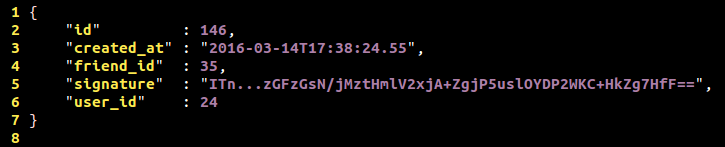
\includegraphics[clip,scale=0.575]{images/signature}
\par\end{center}%
\end{minipage}}

\protect\caption{Vertrauensbeziehung zwischen zwei Benutzer}


\end{figure}


Unterschied zu PGP bzw. OpenPGP wird eine weniger komplexer immerhin
informative Daten abgepeichert zur Materialiesierung von Vertrauenbeziehung
zwischen zwei Benutzer. Eine Vergleich von die beide Vertrauenbeziehungmaterialisierung
zeigt der Abb. \ref{untershied zu pgp-zertifikat}

\label{untershied zu pgp-zertifikat}
\begin{figure}
\begin{minipage}[t]{1\columnwidth}%
%
\end{minipage}

\protect\caption{Unterschied zwischen PGP-Zertifikat und Vertrauenbeziehungsmaterialsierung
in Cryptone}


\end{figure}



\subsection*{Benutzer als Friend hinzufügen}

Sei Alice und Bob zwei Benutzer des Cryptone System. 

Alice möchte Bob als Freund hinzufügen. Eine Friend-Beziehung bzw.
Vertrauenbeziehung zwischen Alice und Bob entsteht wenn das Public-Key
von Bob von Alice signiert wurde und das Public-Key von Alice von
Bob ebenso signiert wurde. 

Die Benutzer die sich in System befinden können sich in eine Freundschaftbeziehung
befinden ( Friends ).\\
Hat Alice Bob als ,,Friend`` hinzugefügt, so können weitere Freunde
von Alice Bob als Friend annehmen. Dadurch bildet sich eine Kette
von ~Friends~ {[}WEB-OF-TRUST{]}. Weitere ist die Freundschaftbeziehung
zwischen Benutzer ein Randbedingung damit A beispielsweise B in eine
Gruppe hinzufügen kann, und mit B dann auch Dokumenten durch von A
gegründete Gruppe austauschen kann.\\
Bei der Herstellung eine Vertrauensbeziehung ( Friend ) zwischen A
und B , wird die öffentliche Schlüssel B von A signiert. diese Signatur
bildet materialistisch die Vertrauensbeziehung zwischen A und B. \\
Die Signatur spielt nicht nur eine Rolle, um der Vertrauensbeziehungsherstellung
zwischen zwei Benutzer, sondern auch beim Überprüfung von RemoteServer
Integrität. Log sich ein Benutzer ein und merkt dass seine Signaturen
nicht mehr stimmen, dann wurde der RemoteServer kompromittiert. 


\subsection*{Vertrauensbeziehung zurückziehen}


\section{Übermittlung von Passphrase }

Passphrase wird übers Handy durch RemoteServer an der LocalServer
weitergeleitet. Dank diese Massnahme wird eine Gefahr abgelöst, und
zwar das Gefahr dass ein KeyLogger auf der Computer installiert ist.
Aus diesem Grund ist es sinnvoll das Passphrase durch eine andere
Kanal zu übermittelt. Das ganze sollte keine zusatzliche Softwareinstallation
benötigen, spricht die Übermittlung von Passphrase sollte per Browser
geschehen, und zwar ein Handybrowser.\\
Wie in Abschnitt \ref{sec:local_server_public_key} gesehen, wird
beim Start der LocalServer ein Schlüsselpaare erzeugt, der ~CLIENT\_PUBLIC\_KEY~
wird dann als Header gesetzt, und der geheime Schlüssel bleibt an
LocalServer. diese öffentliche frisch generierte Schlüssel ist nicht
mit der Benutzerschlüssel zu verwechselt. Die öffentliche Schlüssel
der als Header gesetzt wurde und von daher systemweit zugreifbar ist
kann an der Handy geschickt wird, und von dort aus wird von der Benutzer
eingegeben Passphrase mit der ~CLIENT\_PUBLIC\_KEY~ verschlüsselt.
die mit der öffentliche Schlüssel verschlüsselte Passphrase gehe dann
von Handy zur LocalServer über RemoteServer.


\section{Gruppe }

Gruppe in Code Dokumentation ,,Group`` ist eine wichtige Konzept
in Cryptoone-System. Gruppe ist das Konzept was Benutzer miteinander
verbindet zufolgedessen Dokument und Schlüssel. \\
Zu eine Gruppe gehört eine Schlüsselkey ( Symmetrische Schlüssel )
, abgekürzt GK, da diese Schlüssel eine kritische Information ist,
taucht der nicht unverschlüsselt in RemoteServer. Beim Erstellen einer
Gruppe beim einem Benutzer wird der KG mit der öffentlichen Schlüssel
der Benutzer verschlüsselt, zu einer Gruppe gehört genau einer KG. 

Eine Gruppe kann genau einen ( Private Gruppe PG ) , genau zwei (
Eins-zu-Eins-Gruppe EZEG ) oder 1 bis mehrere Mitglieder ( öffentliche
Gruppe OG ) haben. \\
Der Gruppeverantwortlich kann jederzeit der Gruppe löschen, und zwar
ganz unabhängig von der Art der Gruppe.


\section{Dokumentaustausch}


\subsection*{von private Gruppe zu öffentliche Gruppe }

das Teilen eines Dokuments lässt sich in verschiedene Weise durchführen.
Ein Benutzer kann ein Dokument per Upload in seine private Gruppe
hochladen. Das Dokument bleibt in seine private Gruppe solange bis
der Benutzer die Entscheidung trifft das Dokument mit eine andere
Gruppe zu teilen. Ab dann gehört das Dokument nicht mehr der Benutzer,
dass heisst der kann das Dokument nicht mehr zurückziehen, ausgeschlossen
der Benutzer ist der Gruppeverantwortlich der Gruppe, dann kann der
wieder das Dokument zurückziehen. Das Original des von neulich in
eine öffentliche Gruppe geteilte Dokuments bleibt aber im Benutzer
private Gruppe.

\begin{figure}
\fbox{\begin{minipage}[t]{1\columnwidth}%
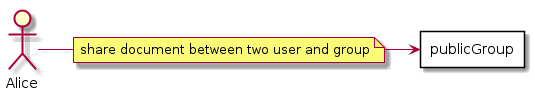
\includegraphics[scale=0.8]{images/src/pu/usecase/user_to_group_document_share}%
\end{minipage}}

\protect\caption{Zwischen Benutzer und Group}


\end{figure}



\subsection*{zwischen zwei öffentliche Gruppe}

Ein Dokument der sich in eine öffentliche Gruppe befinden kann mit
einer anderen Gruppe geteilt werden, vorausgesetzt dass der Gruppeverantwortlich
auch in der zweite Gruppe Mitglied ist. 

\begin{figure}
\fbox{\begin{minipage}[t]{1\columnwidth}%
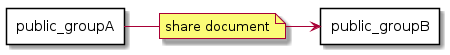
\includegraphics[scale=0.9]{images/src/pu/usecase/share_with_group}%
\end{minipage}}

\protect\caption{Public Group zu Public Group}


\end{figure}


Ablauf : 
\begin{enumerate}
\item Dokument D in Gruppe A 
\item Prüfen ob Benutzer U GV in Gruppe A 
\item Prüfen ob GV , Gruppemitglieder in Gruppe B 
\item authorizieren das Teil von Dokument D zwischen Gruppe A und B
\end{enumerate}

\subsection*{Zwischen zwei Benutzer }

Ein Benutzer A kann sich entscheiden ein Dokument D nur mit einer
Ihrer Freund B zu teilen. Ist der Benutzer B noch keiner Freund von
A, dann wird während dieser Vorgang B als Freund von A vertraut gemacht
( Das heisst während dieser Vorgang der Benutzer B öffentliche Schlüssel
wird von Benutzer A signiert ). Eine Gruppe wird dann erzeugt und
das zu auszuteilenden Dokuments wird in der neulich erzeugte Gruppe
verwiesen. der Benutzer B muss dann die Freundschaftanfrage von A
bestätigen schliesslich darf er auf Dokument D zugreiffen. \\
Wie auf der unterstehende Abbildung \ref{fig:Benutzer-Benutzer-Dokumentsaustausch}
zu sehen ist, der Benutzer der den Vorgang auslöst wird dann als Gruppeverantwortlich
der zu erzeugende Gruppe markiert, in der Fall Benutzer Alice. Alice
kann jeder Zeit die Gruppe wieder löschen oder Bob von der Gruppe
entfernen. 

\begin{figure}
\fbox{\begin{minipage}[t][0.05\paperheight]{1\paperwidth}%
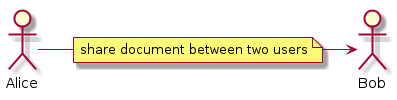
\includegraphics[scale=0.8]{images/src/pu/usecase/user_to_user_document_share}%
\end{minipage}}

\fbox{\begin{minipage}[t]{1\paperwidth}%
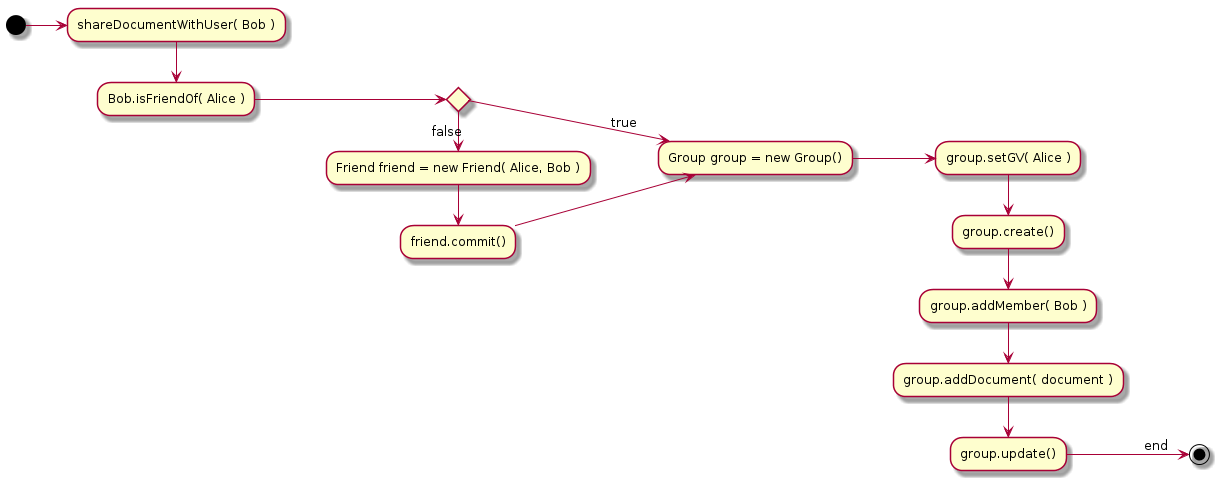
\includegraphics[scale=0.4]{images/src/pu/activity/user_user_document_share}%
\end{minipage}}

\protect\caption{\label{fig:Benutzer-Benutzer-Dokumentsaustausch}Benutzer-Benutzer
Dokumentsaustausch}
\end{figure}



\section{REST (Representational State Transfer)}

Es darf systemweit HTTPS nicht im Einsatz kommen und/oder Einsatz
von zustand behaftete Verbindung ( Session ). Ein sehr geschickte
Konzept um diese Anforderung zu erfüllen ist der REST-Konzept. Der
REST-Konzept besagt dass eine Anfrage alle Informationen zur vollständige
Bearbeitung der Anfrage beinhalten muss. die Anfrage benutzen explizite
Http Methode ( GET, POST , PUT, DELETE ), und die auf der Server zur
Verfügung gestellte Resource haben eine Dokument ähnliche Organisation.
\\
Beim Einsatz von REST wird kein ~Query String~ benutzt, was als
Vorteil hat, eine mögliche Sicherheitlücke zu vermeiden. Eine weitere
Vorteil ist die Überschaubarkeit der Software.

\begin{figure}
\fbox{\begin{minipage}[t]{1\columnwidth}%
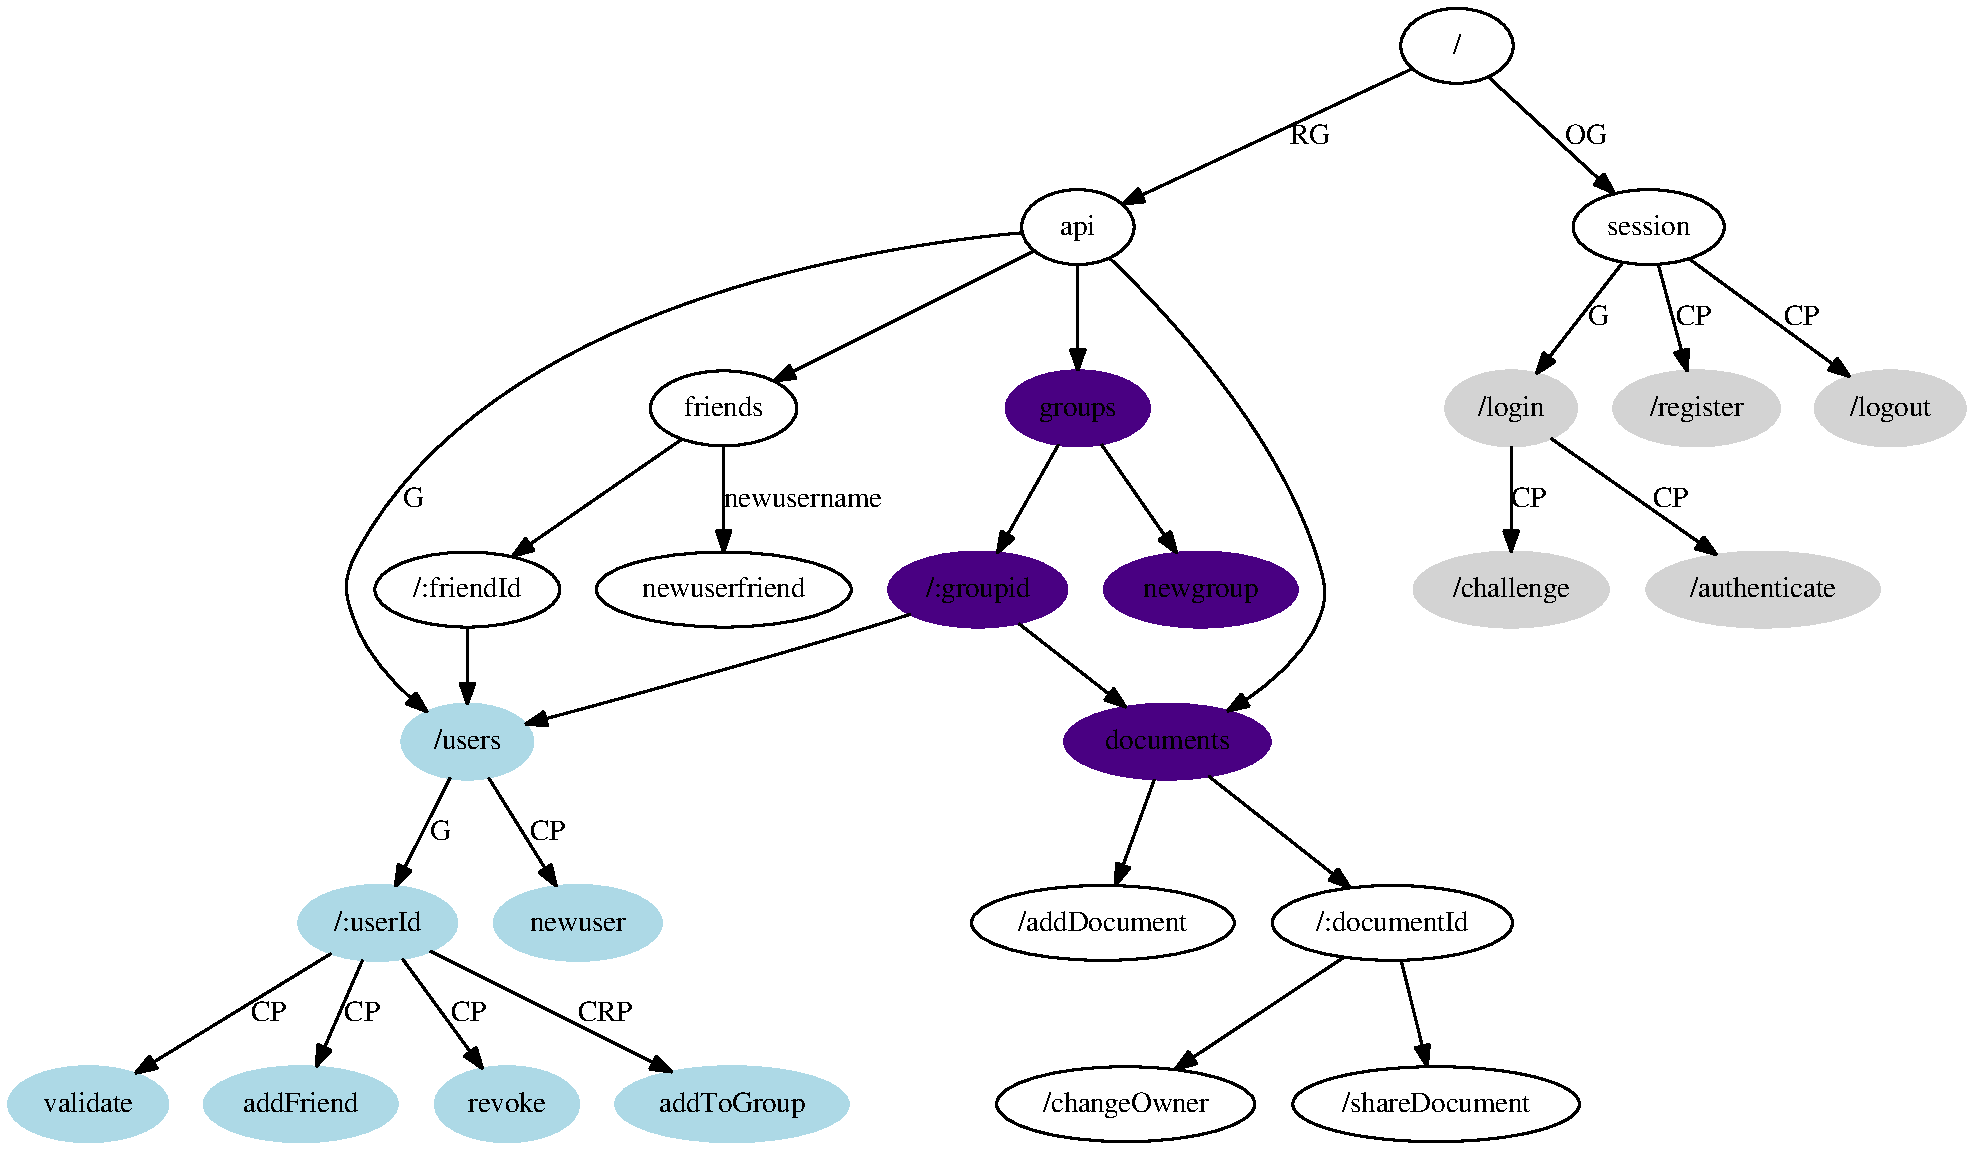
\includegraphics[clip,angle=90,origin=lb,scale=0.6]{images/src/dotty/routes}%
\end{minipage}}

\protect\caption{Routes/Aktionen}


\end{figure}



\section{Integrität der transportierte kritischen Daten ( JWS )}

Bei sicherheitsrelevanten Software ist es wichtig die Daten zu verschlüsseln
mit einem konsequent Schlüssellänge, und die Integrität diese Schlüssel
gewährleistet. Diese gilt und ist ausreichend solange die Daten und
Schlüssel nicht über Internet beispielerweise transportiert werden.
Wenn die Daten über eine unsichere Neztwerk übermittelt werden muss
eine zusätzlicher Integritätmechanismus im Spiel kommen, um sicherzustellen
dass eine Daten die von A zu B beispielerweise transitiert, unterwegs
nicht verfälscht wurde.\\
Als Lösungsatzt wird eine End-to-End Integritätsprüfung eingesetzt
mithilfe der JWS ( JSON Web Signature ) spezifiziert in RFC 7515\cite{JWS}\\
JWS basiert auf JSON Web Encryption (JWE)\cite{JWE} um kryptographische
Operationen durchzuführen. JWE implementiert die meistens bekannte
standard kryptographie Algorithmus, wie RSA, AES ....\\
JWS benutzt die von JWE implementiert RSA um Daten zu signiert. Bei
Einsatzt von JWS muss Acht darauf gegeben dass die JSON-Daten richtig
formatiert wurde. 

exemplarische JWT Headers:

\begin{figure}
\begin{tabular}{|c|c|c|}
\hline 
 & Headername & Beschreibung\tabularnewline
\hline 
\hline 
1 & alg & Name der kryptograpschische Algorithmus\tabularnewline
\hline 
2 & hash & hash Wert\tabularnewline
\hline 
3 & typ & Mediatyp\tabularnewline
\hline 
4 & jwk & JSON Web Key\tabularnewline
\hline 
\end{tabular}

\protect\caption{JWS Header}
\end{figure}


JWS stellen weitere Headers zur Verfügung, aber die werden Anhand
diese Arbeit nicht benutzt. Die Header werden gesetzt bei der letze
Filter. In diese Signature-Filter, wird die von Controller bereitgestellte
Inhalt dessen Hash berechnet und gegebenfalls auch signiert (nicht
alle Daten mussen signiert werden). 

\begin{figure}
\fbox{\begin{minipage}[t]{1\columnwidth}%
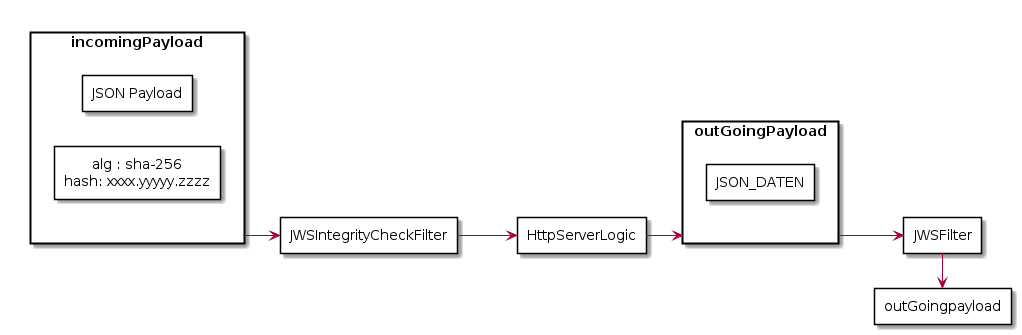
\includegraphics[scale=0.35]{images/src/pu/usecase/filter_signature}%
\end{minipage}}

\protect\caption{JWS Filter}


\end{figure}



\section{JSON Web Token (JWT) }

\begin{figure}
\fbox{\begin{minipage}[t]{1\columnwidth}%
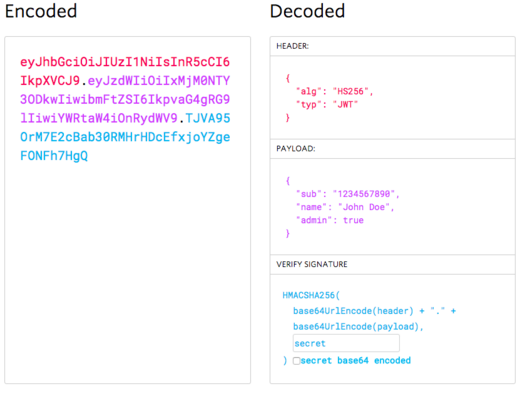
\includegraphics[scale=0.8]{images/jwt}%
\end{minipage}}

\protect\caption{Json Web Token}


\end{figure}


JWT ist eine JSON-basierte Standard um Authentication-Objekt zu repräsentieren.
Eine Anwendungsfall ist beispielerweise OpenID-Authentication. Es
erlaubt einem Benutzer, der sich bei seinem sog. AuthenticationProvider
einmal mit der Benutzername und Passwort angemeldet hat, sich nur
mit Hilfe erhaltene JSON Web Token (JWT) ohne Benutzername und Passwort
bei allen das System unterstützenden Websites anzumelden. wobei man
sich gegen ein Authenticationserver A authentifizieren kann, den erhaltene
Token wird dann später anhand eine Anfrage an ResourceServer benutzt.
\\
Token werden an Stelle von Benutzername-Passwort-Kombinationen verwendet,
um auf Ressourcen zuzugreifen. Ein Token ist meist eine Zeichenkette
aus Buchstaben und Zahlen; Sonderzeichen können auch verwendet werden.
Um es vor Missbrauch zu schützen soll es schwer zu erraten und passend
zu einer Sicherheitsabfrage sein. OAuth unterscheidet zwischen Abfrage-Token
und Zugangs-Token.


\section{Notar (SGK zurückgewinnen)}

In Falls das System wird unsicher, nach Entdeckung zum Beispiel eines
verfälschten öffentlichen Schlüssel, wird alle Informationen in Datenbanken
und dabei alle Schlüssel gelöscht. Es sollte eine Möglichkeit gegeben,
die Dateischlüssel zurückzugewinnen. Deswegen wird in System den öffentlichen
Schlüssel eines Notars eingeführt. Bei Hochladen eines Dateien wird
eine Kopie des symmetrischen Schlüssels des Dateien mit dem Notar
öffentlichen Schlüssel verschlüsselt. Nach Meldung eines Problems
im System, wie fehlerhaftes oder falsches Signatur beziehungsweise
öffentlichen Schlüssel, können alle SGK anhand des Notar privaten
Schlüssel entschlüsselt werden und damit alle Dateien zurückgewinnen.Hier
ist es wichtig zu notieren, dass der Notar private Schlüssel ist nicht
in System gespeichert, sondern in eine sichere Ort außerhalb des Systems.
Nach Generierung ihres Schlüssel-paar müssen alle neuen Benutzer den
Notar öffentlichen Schlüssel signieren und bei jeder Anmeldung seiner
Integrität prüfen. Dadurch wird seine Integrität gewährleisten.


\section{Szenarien}

Hier werden einige Szenarien dargestellt und dazu sequentielle Diagramms,
um die Interaktionen zwischen die einzelne Komponente zu verdeutlichen. 


\subsection*{Benutzer registrieren}

\begin{figure}
\fbox{\begin{minipage}[t]{1\columnwidth}%
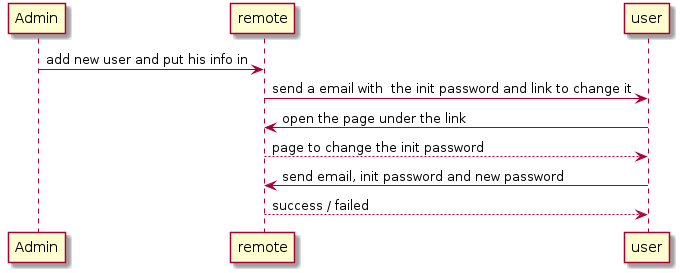
\includegraphics[scale=0.5]{images/src/pu/sequence/registration}%
\end{minipage}}

\protect\caption{Benutzer registration sequence diagramm}
\end{figure}



\subsection*{Benutzer einlogen}

\begin{figure}
\fbox{\begin{minipage}[t]{1\columnwidth}%
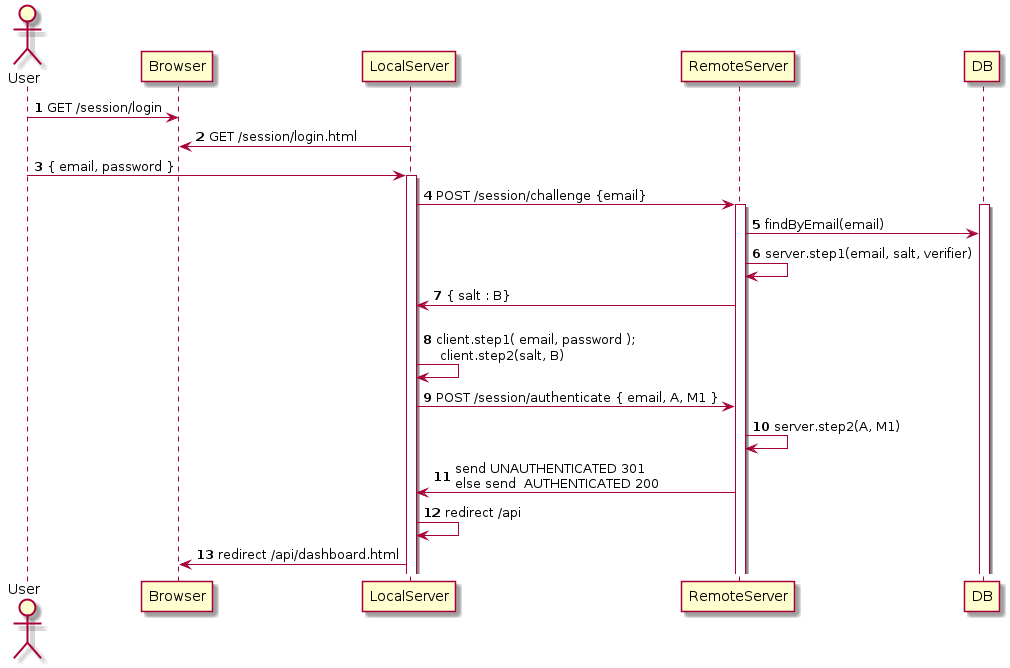
\includegraphics[scale=0.4]{images/src/pu/sequence/login}%
\end{minipage}}

\protect\caption{Benutzer einloggen sequence diagramm}
\end{figure}



\subsection*{Freund hinzufuegen}

\begin{figure}
\fbox{\begin{minipage}[t]{1\columnwidth}%
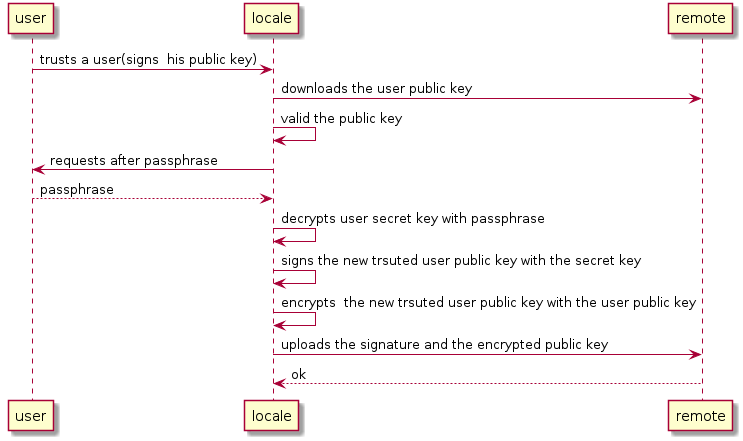
\includegraphics[clip,scale=0.5]{images/src/pu/sequence/trust_a_new_user}%
\end{minipage}}

\protect\caption{Freund hinzufuegen sequence diagram}
\end{figure}

\begin{itemize}
\item Beispielszenario: Alice will Bob als Freund markieren \\
Alice forder die Benutzerlisteseite auf, clicke auf den ,,+`` (
Plus )-zeichen, um Bob als Freund hinzuzufügen.
\item Alice ist gefordert, Ihre Passphrase einzugeben (Falls Passphrase
noch nicht vorhanden ist) 
\item Der LocalServer lädt Bobs öffentlichen Schlüssel von RemoteServer
herunter.
\item LocalServer lädt Alice private Schlüssel vom RemoteServer herunter
(Falls noch nicht vorhanden) und entschlüsselt der letze mit Alice
Passphrase
\item Bobs öffentlichen Schlüssel wird mit Alices privaten Schlüssel signiert. 
\item Aus Signature, Alices und Bobs Id wird ein ,,Friend`` Objekt erzeugt.
Dies entspricht die Vertrauenbeziehung zwischen Alice und Bob. Diese
Objekt wird an RemoteServer geschickt und dort gespeichert.
\end{itemize}

\subsection*{Freund revoke}

Alice will Bob von seine Vertrauenbeziehungen rausnehmen

\begin{figure}
\fbox{\begin{minipage}[t]{1\columnwidth}%
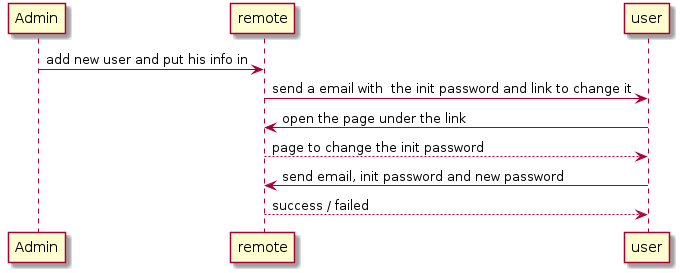
\includegraphics[scale=0.6]{images/src/pu/sequence/revoke_signature}%
\end{minipage}}\protect\caption{Freund revoke sequence diagramm}
\end{figure}

\begin{itemize}
\item Alice fordert die Freundelisteseite auf, clicke auf den ,,-`` (
Minus )-zeichen, um Bob als Freund hinzuzufügen.
\item Alice ist dann gefordert, die Aktion zu bestätigen
\item Bestätigt Alice die Aktion, dann wird die revoke-Request über LocalServer
zu RemoteServer weitergeleitet
\item Auf der RemoteServer wird die Eintrag was die Freundschaft zwischen
Alice und Bob gelöscht
\item Alice wird über die erfolgreiche Zerstörung einer Vertrauenbeziehung
mit Bob informiert.
\end{itemize}

\subsection*{Datei hochladen}

\begin{figure}
\fbox{\begin{minipage}[t]{1\columnwidth}%
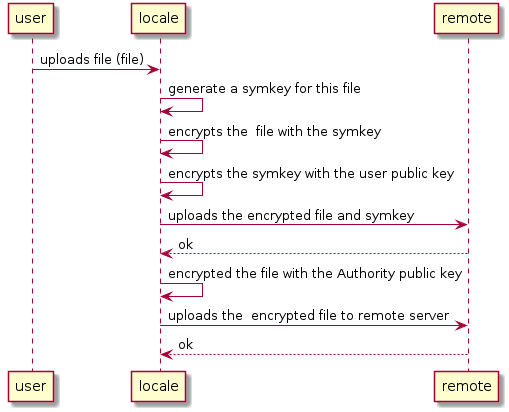
\includegraphics[scale=0.5]{images/src/pu/sequence/upload_file}%
\end{minipage}}

\protect\caption{Datei hochladen sequence diagramm}
\end{figure}

\begin{itemize}
\item Alice will eine Datei hochladen
\item Alice wählt sich eine Gruppe aus wo sie mitglied ist
\item Alice clickt auf Datei Upload und wählt sich Datei aus, die sie gerne
in die vorherige ausgewählte Gruppe hinzüfügen will
\item Alice Clickt auf dem Button ,,upload`` ( hochladen )
\item Die Anfrage wird an LocalServer weitergeleitet
\item Alice Passphrase wird gefördert falls noch nicht im LocalServer vorhanden
ist
\item Alices Schlüsselpaare wird von RemoteServer runtergeladen sowie von
Alice ausgewählte Gruppe Secret Key (SGK)
\item Alice Kopie von SGK wird mit Alice private Schlüssel dechiffriert
\item mit der dechiffriert SGK wird die Datei verschlüsselt. Dechiffriert
SGK wird bald als die Verschlüsselung von Datei erfolgt hat von LocalServer
zerstört.
\item Schliesslich wird die chiffriert Datei zu RemoteServer übermittelt
und ein Eintrag von Typ Dokuments auf der Datenbank gespeichert.
\end{itemize}

\subsection*{Datei herunterladen}

\begin{figure}
\noindent \begin{centering}
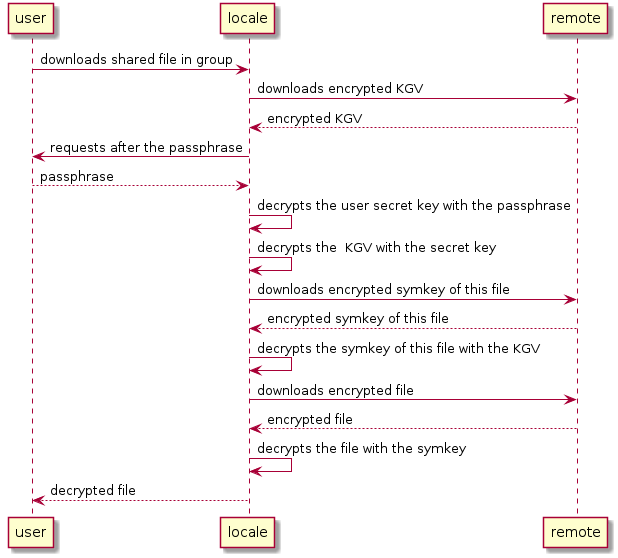
\includegraphics[clip,scale=0.6]{images/src/pu/sequence/download_file_from_group}
\par\end{centering}

\protect\caption{Datei herunterladen}


\end{figure}

\begin{itemize}
\item Alice befindet sich in einer Gruppe und will ein Datei runterladen.
Also Alice muss mitglied von der Gruppe sein
\item Alice click auf ,,download`` (herunterladen), Die Anfrage wird dann
an LocalServer weitergeleitet
\item Alice Passphrase wird gefördert falls noch nicht im LocalServer vorhanden
ist
\item Alices Schlüsselpaare wird von RemoteServer runtergeladen sowie von
Alice ausgewählte Gruppe Secret Key (SGK)
\item Alice Kopie von SGK wird mit Alice private Schlüssel dechiffriert
\item LocalServer lädt von RemoteServer der geförderte Datei runter.
\item Datei wird mit dechiffrierte SGK entschlüsselt. 
\end{itemize}

\subsection*{Neue Gruppe erzeugen}

Alice will eine neue Gruppe anlegen

\begin{wrapfigure}{o}{0.5\columnwidth}%
\fbox{\begin{minipage}[t]{1\columnwidth}%
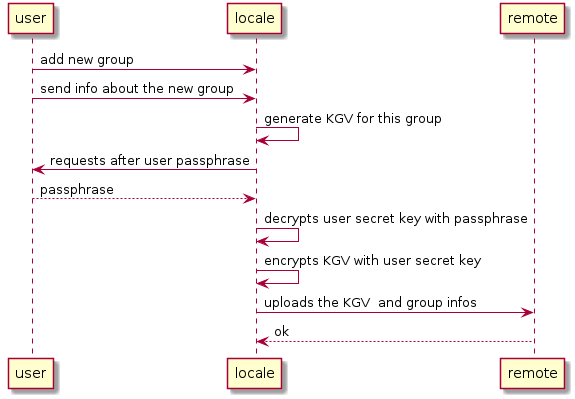
\includegraphics[scale=0.6]{images/src/pu/sequence/new_group}%
\end{minipage}}\protect\caption{Neue gruppe anlegen}


\end{wrapfigure}%

\begin{itemize}
\item Alice klickt auf eine neue Gruppe an und gibt den Name der neuen Gruppe
im ersheinte Pop-up
\item LocalServer lädt Alice öffentliche und private Schlüssel runter.
\item Alice wird gefordert, Ihre Passphrase einzugeben (Falls noch nicht
vorhanden)
\item Es wird eine symmetrische Schlüssel (SGK) 
\item SGK wird mit Alice öffentliche Schlüssel verschlüsselt. 
\item SGK wird mit Alice private Schlüssel signiert. 
\item Nach die vorherige Vorgang, werden ein Gruppe Objekt und SymKey Object
erzeugt. Die beide Objekte werden von LokalServer zu RemoteServer
geschickt.
\end{itemize}

\chapter{Implementierung und Evalierung}

Bei diese Abschnitt geht es um die konkrete Implementierung von der
verschiedenen Softwareteils, nämmlich : 
\begin{itemize}
\item LocalServer 
\item RemoteServer 
\item CryptUtils 
\item Frontend 
\item Inbetriebnahme-programm
\end{itemize}
Es wird als erste eine Unterkapitel über die wesentliche Technologien
die für die Anfertigung des Projektes benötigt wurde, gefolgt von
deren Beschreibung. Insbesondere wird Wert auf die Funktionalität
von die Framework gelegt, die eine bedeutende Role in der Implementierung
haben, und die Gewährleistung von relevante Sicherheitmechanismen
zur Erfüllung die vorgegebene Anförderungen.


\section{Überblick auf die Technologie}

\begin{table}
\begin{tabular}{|c|c|c|c|}
\hline 
 & Programmiersprache & Technologie/Framework & Buildtools\tabularnewline
\hline 
\hline 
CryptUtils & JAVA & JCE, Guava & Maven\tabularnewline
\hline 
RemoteServer & JAVA & Spring, Hibernate, Guava & Maven\tabularnewline
\hline 
LocalServer & JAVA & Spring, Guava & Maven\tabularnewline
\hline 
Frontend & JavaScript/HTML/CSS & AngularJS & GruntJS\tabularnewline
\hline 
\end{tabular}

\protect\caption{Technologie-Überblick}


\end{table}



\section{Allgemein Designentscheidungen}


\subsection{JSON-Format}

Systemweit wird JSON-Format bevorzugt um die Daten zwischen die verschiedene
Softwarekomponente zu transpotieren. Explizit ausgedruckt, heisst
es dass alle High-end Funktionen bzw. die Funktion die durch eine
eine Softwarekomponent zur aussenwelt verfügbar gemacht wurden exportieren
Daten in JSON-Format. Diese Entscheidung lasst sich bei der Interoperabilität
gründen, sowie auch Kriterien wie Einheitlichkeit von Softwareschnittstellen,
was bei der Weiterentwicklung von grossen Bedeutung ist. Durch den
Einsatz von JSON als Export-Format wird beispielerweise das Ersetzen
von Softwarekomponent einfach. Beim Einsatz von JSON wurde die von
Google entwickelte GSON Bibliothek benutzt.


\subsection{UTF-8 und Base64}


\subsection{HTTP Headers}

Headers sind mächtige Werkzeuge wenn es zum Internet kommt, und wichtiger
noch im Bereich Security von Webbasierte Anwendungen. Bei der Entwurf
von dieser Arbeit, wurde die Entscheidung getroffen soviel wie möglich
auf die Standard zu halten, insbesondere bei sicherheitrelevante Bereiche.
Die richtige Einstellung/Konfiguration von manche Headers tragen wesentlich
bei, um der Sicherheitgrad eine Webanwendung zu erhöhen. Es wird nochmal
über Headers die Rede sein, bei alle Softwareteil wo sie gesetzt bzw.
geprüft werden ( LocalServer, RemoteServer, Frontend ), aber hier
ist schon mal wichtig darüber zu erwähnen und eine gesamte Überblick
über die Headers die Systemweit eingesetzt werden.

\begin{table}
\begin{tabular}{|c|c|c|c|c|}
\hline 
Headername & Wert & gesetzt bei & Laufzeit & \tabularnewline
\hline 
\hline 
Content-Security-Policy & script-src 'self' & LocalServer & Erste Request an LocalServer & 1\tabularnewline
\hline 
Authorization & SRP & LocalServer & Erste Login Request & 2\tabularnewline
\hline 
WWW-Authenticate & SRP & LocalServer & Erste Login Request & 3\tabularnewline
\hline 
realm & realm & LocalServer & Erste Login Request & 4\tabularnewline
\hline 
hash-algorithm & SHA256 & LocalServer & Erste Login Request & 5\tabularnewline
\hline 
X-XSRF-TOKEN & ==== & LocalServer & Erste Request an LocalServer & 6\tabularnewline
\hline 
AUTH-TOKEN & ==== & RemoteServer & Nach erfolgreichen Authentifizierung & 7\tabularnewline
\hline 
EXPIRES-IN & ==== & RemoteServer & Nach erfolgreichen Authentifizierung & 8\tabularnewline
\hline 
Client-Public-Key & ==== & LocalServer & Erste Login Request & 9\tabularnewline
\hline 
Server-Public-Key & ==== & RemoteServer & Erste Login Request & 10\tabularnewline
\hline 
typ & JWT & RemoteServer & Nach erfolgreichen Login & 11\tabularnewline
\hline 
alg & RS512 & RemoteServer & Nach erfolgreichen Login & 12\tabularnewline
\hline 
\end{tabular}

\protect\caption{Headers }
\end{table}

\begin{itemize}
\item (1) Content-Security-Policy spiel eine bedeutende Rolle um XSS-Attack
zu vermeiden. mit dem Wert script-src 'self' weist die Header hin,
dass alle JavaScript source Datei nur von Server geladen werden dürfen.
In unsere Fall vom LocalServer.
\item (2) (3) (4) und (5) Informieren den Webbrowser über dem Authentication
Algorithmus bzw. dem Hash-Algorithmus, der eingesetzt wird.
\item (6)Wichtige Header gegen XSRF-Attacke (Cross Site Request Forgery)\footnote{XSRF : Manipulation von Parametern, so dass im Browser Skriptcode
ausgeführt wird; häufig auch synonym zu HTML-Injection verwendet\cite{XSS}}
\end{itemize}

\section{Frontend}

In diesem Kapitel handelt es sich um der Clientoberfläche in Form
eine Webapplication, die der Endbenutzer auf irgendeinem Rechner der
über eine Webbrowser verfügt aufrufen kann. Hier ist noch mal zu erinnern,
dass eine der wichtige Anforderung von dieser Arbeit war das der Software
so konzipiert wird, dass es kein zusätzliche Softwareinstallation
benötigt wird. Das Webapplication wurde in Form eine sog. Single Page
Application, wie bereits erwärnt, handelt es sich um eine Technik
Webseite zu entwerfen, so dass die Bedinung von Webapplication ähnlich
ist wie von Benutzer schon bekannt Computersprogramm. Neben der Usability
und Portierungsargumente kommt auch die strenge Haltung von wichtigen
Softwarearchiktekture und Regeln die mit Einsatz von AngularJS verbunden
sind, nämmlich Separation of Concern und MVVM . Ausserdem ermöglicht
angular eine wesentliche Reduzierung von Request an Server, dass hat
zur Folge dass der ~Man-in-the-middle~ ehe wenige Material bekommt
um eine ~Offline-attacke~ dürchzuführen. 


\subsubsection{AngularJS und Security}

An der Webbrowser wird vorwiegend Angularjs eingesetzt. Was Sicherheit
angeht, werden nämmlich den Angular Speicher strategie, ~cookies~
, die über den angular-service einsetzbar ist. 

\begin{figure}
\begin{lstlisting}
      
var options = 
{
 	secure : true
};

function refresh_storage(){
        var d = new Date( Auth.getHeader( EXPIRES_TOKEN ) );
        var n = d.toUTCString().toString();
        options.expires = n;
}
\end{lstlisting}


\label{code:angular-cookie}\protect\caption{Angular: Cookie Konfigurierung}
\end{figure}


Was path und domain angeht wurden die Default Werte gelassen, und
zwar Cookie steht zur Verfügung für aktuelle Pfad und alle untergeordnete
Pfäder bzw. Cookie steht zur Verfügung nur für die Application domain.
Was hier konfiguriert wurde war den Parameter secure mit den wert
true und expires mit eine Date Instance in Form eine Zeichenkette,
der konfigurierte die Lebensdauer der Cookies. Zusammengefasst darf
nur der aktuelle Angular Application auf der Cookies zugreifen, und
der Lebensdauer von der Cookie wird von Angular managiert. in der
Abbildung \ref{code:angular-cookie} wird die in Cookie gespeicherte
Daten nach Sechs Minute zerstört,infolgedessen der Benutzer automatisch
ausgeloggt wird. die Ablaufzeit wird von der Server bestimmt und über
der Header ,,EXPIRES\_IN`` zur LocalServer bzw. zur Angular Applikation
übermittelt.


\subsection{Ausstatung von Routes}

Die unterstehende Grafik repräsentiert die mögliche Aktionen, die
den Be- nutzer mithilfe der Webbrowser auslösen kann. Es lass sich
dadurch nochmal eine graphische abstrahierende Darstellung von funktionale
Anforderungen darstellen.

\begin{wrapfigure}{o}{0.5\columnwidth}%
\protect\caption{Routes-Übersicht}
\end{wrapfigure}%



\section{allgemeine Implementierung Entscheidung von Local-und Remoteserver}

Beide LocalServer und Remoteserver wurde in Java mithilfe der Framework
Spring programmiert. Spring ist eine allgemeine Zweck Framework um
Desktop- sowie Internetbasierte Anwendungen zu implementieren. Folgedessen
ist Spring meistens eng mit Internet bezogene Context verbunden, was
das Testen von Software behindert oder sogar nicht möglich macht. 


\section{LocalServer}

LocalServer wurde konzipierte um in ein USB-Stick laufähig zu sein,
und zwar ganz unerterschieden von Betriebsystemart\footnote{Jetzige Stand von LocalServer wurde auf Linux basierte Betriebsystem
und Window Betriebsystem erfolgreich getestet.} . Das Ziel wurde erreicht indem dass LocalServer mit Java programmiert
wurde. Das Programm an sich und eine lauffähige JVM liegen dann in
der USB Stick. \\
Auch wenn LocalServer mit einem Plattform unabhängige Programmiersprache
implementiert wurde, musste nochmal dass Programm rücksichtvoll konfiguriert
werden, damit beispielerweise Der LocalServer nicht auf ein Port zuweisen
den schon für ein andere Zweck auf der Benutzerrechner belegt wurde.
\\



\section*{LocalServer Module}


\subsubsection*{CryptoUtils}

Diese Module enthält alle kryptographische Funktionalitäten, welche
für diese Arbeit eine Rolle spielen, nämlich : 
\begin{enumerate}
\item Symmetrische Verschlüsselung und symmetrische Schlüssel-Generator. 
\item Asymmetrische Verschlüsselung und asymmetrische Schlüssel-Generator
\item Passwort basierte asymmetrische Schlüssel-Generator
\item Digitale Signature
\item Hashwert-Berechnung
\item Zufall-Generator (Salt-Generator) 
\end{enumerate}
Alle oben genannte Funktionalität wurden als Funktionsmodule (Gedächtnislose-Module)
implementiert. Schlüssellänge und eingesetzte Algorithmus können durch
die Konfigurationsdatei geändert werden.\\
Die obengennante Untermodule verfügen über eine einheitliche Schnittstelle,
Parameter-Typ und Rückgabewert sind immer Base-64 codierte JSON-Zeichenkette.
\\


\begin{figure}
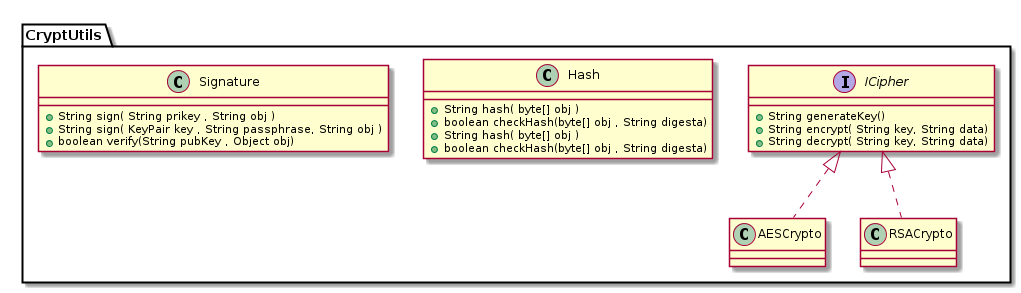
\includegraphics[clip,scale=0.5]{images/src/pu/class/crypto}

\protect\caption{Klasse-diagramm CryptoUtils}


\end{figure}


Alle Klasse werden sowie in der oben stehenden Abbildung weiter im
LocalServer benutzt (,,AS IS``). Ausnahmeweise wird AESCrypto abstrahiert
um eine Spezialisierung für Dateiverschlüsselung zu entwerfen. 


\subsection*{Konfigurationsdatei}

\begin{figure}
	\lstinputlisting[emph={remoteserver, url, uri, maxFileSize, register, login, authenticate, users, documents, groups, friends, port, app, server, multipart, keypairs, symkeys, name, description, maxRequestSize, logout, challenge},emphstyle={\color{green}},caption={application.yml},label={Konfigurationsdatei}]{samples/application.yml}

\protect\caption{Konfigurationsdatei }
\end{figure}
\label{sub:konfiguration_localserver}

Abbildung \ref{sub:konfiguration_localserver} zeigt eine exemplarische
Spring-Boot Projekt Konfiguration wie es in den Projekt eingesetzt
wurde. Spring-Boot übernimmt die Verwaltung von Konfigurationdatei
und sorgt zur Verbindung von in der Konfigurationsdatei eingetragene
Wert und dessen Verweis im Java Code, oder auch zur Bestimmung der
Kontext. in der oben bennante konfigurationdatei wird zum Beispiel
der Wert Port zu 0 gesetzt, was dafür sorg dass LocalServer immer
eine beim Clientrechner nicht verwendete Port benutzt. Beim RemoteServer
muss dieser Wert jedoch immer fest sein. Weitere werden in Konfigurationdatei
Werte wie Schlüssellänge, Servermessage un Datenbankverbindungsinformationen
festgelegt. Es ist anzudeuten dass die Konfigurationswert von RemoteServer
modifiziert sein können um etwa die Datenbankverbindungsinformationen
auf der RemoteServer anzupassen. Diese modifikation gescheht durch
modifizierung der Konfigurationsdatei oder per commandline-argument
beim aufrufen von ~java~ zur Compilierung.\\

\begin{quotation}
\$ java -jar -Dspring.profiles.active=production CryptoRemote-0.0.1-SNAPSHOT.jar 
\end{quotation}

\subsection*{Model View Controller}

Model view controller (MVC, englisch für Modell Präsentation Steuerung)
ist ein Muster zur Struktierung von Software-Entwicklung in die drei
Einheiten Datenmodell, Präsentation und Programmsteuerung. Ziel des
Musters ist ein flexibler Programmentwurf, der eine spätere Änderung
oder Erweiterung erleichtert und eine Wiederverwendbarkeit. 

Diese Entwurf ist ein Kern-feature von Spring-boot, die verschiedene
Erleichterung bereitstellt für eine einfache Implementierung von Software
nach MVC Modell. Diese Erleichterungen sind zum Beispiel Annotations
wie ,,@RestController`` ,,@Service`` oder auch ,,@Component``. 

\begin{figure}
\fbox{\begin{minipage}[t]{1\columnwidth}%
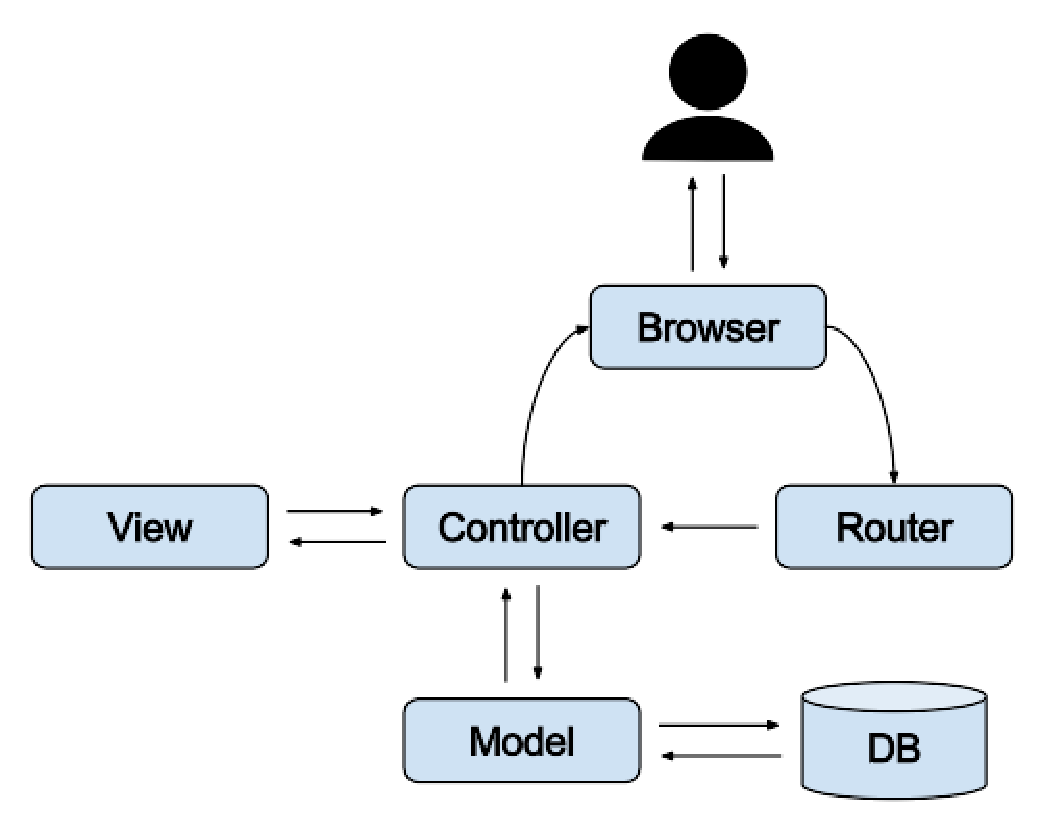
\includegraphics[scale=0.6]{images/MVC}%
\end{minipage}}

\protect\caption{MVC-Muster}
\end{figure}


Der Controller (mit RestController oder Controller Annotation vorgesehen)
ist mit Applikation-Logik (mit Service Annotation vorgesehen) verkoppelt.
Controller-Einheit stellt auch die Ressource zur Außenwelt zur Verfügung.
\\
Applikation-Logik besteht aus zwei Schichten, Controller und Service.
Controller die mit Internet-spezifische Technologie gekoppelt ist
nimmt die Anfragen entgegen. Bearbeitung der Anfrage an sich geschieht
im Service. Dank diese Schichtmodell und Entkopplung von Service und
Controller wird erzielt, dass die Integrationstest der Software ohne
Http-spezifische Softwarekomponente durchgeführt werden kann. 


\subsection*{RestClient }

RestClient Module ist dafür verantwortlich Http-Anfrage an RemoteServer
versenden. 


\subsection*{Fehlerbehandlung und Benutzerrückmeldung}

Fehlerbehandlung ist der Kern ein Softwaresystem. Implizite Anforderungen
beim Entwurf eines Software ist immer eine sinnvolle Rückmeldung an
Benutzer ( Aktion erfolgreich bzw. nicht erfolgreich ). Die Gründe
für eine nicht erfolgreiche Aktion könnten an viele Stelle sein: 
\begin{itemize}
\item Falsche Request
\item momentane nicht ansprechbare Resource
\item Fehler im Code
\end{itemize}
Je nach Fehlerart bzw. Meldungsart, ist es wichtig den Benutzer ein
gewisse Feedback zu geben und schliesslich den Fehler behandeln können
oder dokumentiert für eine nachtragliche Verbesserung des Softwares\\
Anhand dieser Arbeit wurde folgende Http-Status code benutzt :

\begin{figure}
\begin{minipage}[t]{1\columnwidth}%
\begin{tabular}{|c|c|c|c|}
\hline 
 & Status-code & Kurzbeschreibung & Beschreibung\tabularnewline
\hline 
\hline 
1 & 200 & OK & \tabularnewline
\hline 
2 & 201 & CREATED & \tabularnewline
\hline 
3 & 202 & DELETED & \tabularnewline
\hline 
4 & 204  & No Content & \tabularnewline
\hline 
5 & 401 & Error Authentication & \tabularnewline
\hline 
6 & 403 & Forbidden  & \tabularnewline
\hline 
7 & 405 & Not allow & \tabularnewline
\hline 
8 & 400 & ERROR & \tabularnewline
\hline 
\end{tabular}%
\end{minipage}\protect\caption{Http-Status code. RFC2616\cite{HTTPSTATUS} }
\end{figure}


Mit Hilfe von Angular Http Interceptor wurde ein Logik implementiert,
die die Status-code von Http Response filtert, und jenach status code
eine zugehörige Rückmeldung im Browser anzeigt. \\
Sollte ein Fehler Code auftauchen, dann wird automatische eine Antwort
mit Status-Code 500 an Browser geschickt. Diese Sachverhalten ist
aber nicht gewünscht, da es Benutzer und/oder ein eventueller Angreifer
darüber informiert dass beispielerweise ein NullPointer Exception
in Code aufgetaucht wurde. Dies kann der Angreifer benutzen um das
System zu hacken. RemoteServer und LocalServer haben ein Filter, der
die Anwort an Client filtert und 500 Status code durch 400 Status
code ersetzt, weitere wird die verbose Nachricht was die Fehlerquelle
beschreibt durch eine weniger informative Message ersetzt. Alle Code
Fehler, materialisiert durch 500 Status Code werden dokumentiert,
in Log Datenbank und Log-Datei, ein Email mit genau Beschreibung des
Fehlers wird zur Admin geschickt jedes mal das solche Fehler auftauchen. 

\begin{figure}
\fbox{\begin{minipage}[t]{1\columnwidth}%
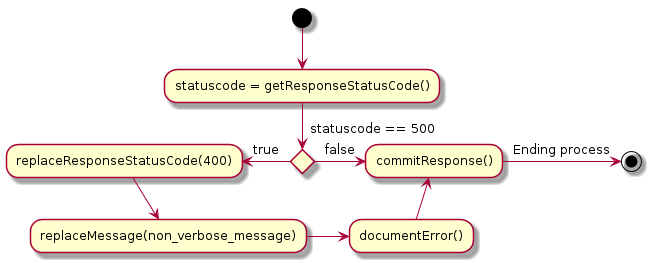
\includegraphics[scale=0.5]{images/src/pu/activity/user_error}%
\end{minipage}}

\protect\caption{Status-Code Filter}


\end{figure}



\subsection*{Caching}

Um häufigere Http-Anfrage an RemoteServer zu vermeiden, wurde eine
Caching-Strategie im LocalServer und Angular Frontend-Application
entworfen. Eine Vorteil von Caching ist es die Overhead zu vermeiden.
Und eventuele ein Dritter der die Kommunikation abhört, nicht durch
häufige Anfrage mit Infos füttert. Caching spielt auch eine beteundente
Rolle bei Skalierung von Software und führt dass die Software mehr
Fehlertorant wird. Caching erbringt mehr Leistung durch eine Verringerung
der durchschnittlichen Latenzzeit von einer einer Reihe von Interaktion
und erhöht die benutzerwahrgenommene Leistung. 

\begin{table}
\fbox{\begin{minipage}[t]{1\columnwidth}%
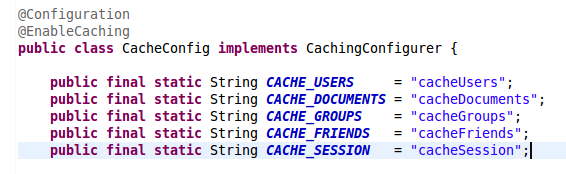
\includegraphics[scale=0.7]{images/cacheConfig}%
\end{minipage}}

\protect\caption{Caching configuration}


\end{table}


Weitere wird Caching benutzt um Session Daten wie zum Beispiel chiffriert
Passphrase zu speichern. Dadürch wird vermeidet dass Benutzer immer
wieder seine Passphrase eingeben muss und eventuelle Keylogger-attacke
vermeidet. 


\section*{Datenbank Schema}

Das unterstehende Abbildung zeigt die Datenbankschema. Dabei ist zu
beachten dass alle als kritischen bzw. sensiblen Informationen mit
zwei wichtige Einträge vorgesehen sind und zwar : ,,hash`` und ,,signature``.
Wie vorher erwarnt, sind diese Einträge wichtig für die Integritätüberprüfung
von Daten.

\begin{figure}
\fbox{\begin{minipage}[t]{0.55\columnwidth}%
\includegraphics[clip,scale=0.6]{images/relationships\lyxdot real\lyxdot large}%
\end{minipage}}

\protect\caption{Datenbank Schema}
\end{figure}


Datenbankschema beschreibung : 
\begin{description}
\item [{Users:}] Im Schemas Users wird die Benutzerinformationen gespeichert
\item [{SrpCredentials:}] In dieser Tabelle werden Benutzerinformations
bezuglich SRP-A, aus Sicherheitgründe wurde diese Informationen vom
Users Schema entkoppelt. 
\item [{Friends:}] Friends ist die Materialsierung von eine Vertrauenbeziehung
zwischen zwei Benutzer. stellt die Vertrauensbeziehung zwischen dem
Benutzer dar. Sobald ein Benutzer den öffentlichen Schlüssel eines
anderen Benutzers signiert, wird eine Zeile in dieser Tabelle eingefügt,
wobei die signority\_id und user\_id die Id der vertrauenden und des
Vertrauten sind.
\item [{Roles:}] Benutzer Roles, die sind festgelegt, wert für eine Role
könnten : ,,Admin`` oder ,,User`` sein. Es ist zu beachten dass
pro Deployment nur ein einziger Benutzer als Admin markiert werden
darf. Weitere Benutzer werden alle als ,,user`` markiert. 
\item [{Session:}] Es handelt sich um die Materialsierung einer aktiven
Session
\item [{UsersGroups:}] Überbrücke zwischen die Tabelle User und Group 
\item [{Groups:}] Hier werden die Informationen relativ zu den Gruppen
gespeichert. Hier ist der Attribute SGK ist der gemeinsam Gruppe Schlüssel
und ist mit dem öffentlichen Schlüssel des Administrators oder Gründer
dieser Gruppe verschlüsselt.
\item [{Documents:}] beinhaltet Dokumenteninformationen. 
\item [{SymKeys:}] Symmetrischen Schlüssel
\item [{PairKeys:}] Assymetrischen Schlüssel.
\end{description}

\section{Evaluierung }

In diesemen Abschnitt wird überprüft, in wieweit die Umsetzung des
Lösungskonzeptes die geforderten Anforderungen an der Cryptone-System
erfüllt. Zusätzlich wird auf Maßnahmen eingegangen, um Korrektheit
des Dienstes sicherzustellen. 


\subsection{Anforderungserfüllung}

Die Anforderungen aus Kapitel \ref{chap:Anforderungen} wurde in in
funktionale und nichtfunktionale Anforderungen unterteilt. Während
die funktionalen Anforderungen durch konkrete softwaretechnische Einheit
(Klasse, Module) werden konnten, beziehen sich die nichtfunktionalen
Anforderungen auf Eigenschaften des Gesamtsystems, die sich mnicht
an einzeilnen Modulen festmachen lassen. \\
Um die funktionalen Anforderungen mit den Modulen abzugleichen, mussten
die einzelnen Anforderungen teilweise in kleinere Schritte unterteilt
werden, um Software besser zu gestalten. \\
Die Kernfunktionalität von Software ( Authentication, Registrierung,
Dateiaustauschoptionen ...) wurde durch eine Unit-Test Programm getestet.
{[}Siehe Anhang für die Ergebnisse{]}, sowie auch nichtfunktionale
Anforderungen wie :
\begin{itemize}
\item Funktionparameter Integrität prüfung ( Null-Object , nicht genug Argument,
falsche Argument, Argumenttyp Prüfung ) 
\item Allgemein Laufzeit Fehler ( Zum beispiel Cryptographie-Algorithmus
nicht Verfügbar ) 
\end{itemize}

\subsubsection{Nicht funktionale Anforderungen : Portabilität}

RemoteServer und LocalServer sollte portable sein. 

\begin{figure}
\begin{tabular}{|c|c|c|c|}
\hline 
 & Nach Kompilierung & Betriebsystem & Laufumgebung\tabularnewline
\hline 
\hline 
LocalServer & JAR & unabhängig & JRE\tabularnewline
\hline 
RemoteServer & WAR & unabhängig & Servlet Container \tabularnewline
\hline 
FrontenApp & JS, HTML & unabhängig & Webbrowser\tabularnewline
\hline 
\end{tabular}

\protect\caption{Cryptone Compilierung}


\end{figure}


die obere Tabelle, zeigt die Verschiede Softwareteile des Projekts,
Alle Softwareteil können ganz unabhängig von Betriebsystem zur Laufen
gebracht werden.Obwohl Die Softwareteilen betriebsystem-webbrowser
bzw. laufumgebungsoftware unabhängig sind, müssen sie eventuelle angepasst
oder zusätzliche Software wie Browser (Internet Explorer hat eine
renomierte Compatibiltät-Problem mit den aktuellten Internet Standard)
installiert werden, aber keinerlei wird eine Softwareänderung benötigt. 

Stand des Tests: 
\begin{itemize}
\item LocalServer läuft auf eine USB-Stick : diese USB-Stick ist mit Java
Runtime Environment (JRE) (64 und 32 Bit) vorgesehen, sowie Windows
JRE (64 Bits), und eine skript ( bash für Linux System und bat für
Window), schliesslich das LocalServer Software an sich. LocalServer
wurde erfolgreich auf Ubuntu 15.10 wily 64 Bits und Windows 7 64 Bits
getestet. 
\item RemoteServer wurde erfolgreich unter Ubuntu 15.10 wily 64 Bits, mit
Apache Tomcat 8.x getestet
\item FrontendApp wurde erfolgreich unter Ubuntu 15.10 wily 64 Bits und
Windows 7 64 Bits mit Webbrowser Google Chrome und Mozilla Firefox
erfolgreich getestet.
\end{itemize}

\subsubsection{Nicht funktionale Anforderungen : Usability}

Trotz die Komplexität des Projektes wurde die CryptoSystem-Client
User-Freundlich wie möglich entworfen. Die Interaktion gescheht durch
eine Webseite. Die mögliche Aktionen (,,sign-in``, ,,sign-up``,
,,upload``, ,,download``, ,,share``, ,,add-friend`` ), Drag-and-Drop
sind üblich und von Benutzer aus andere Webseite bekannt. Fakt ist
dass Zielbenutzer von Cryptone-System sind mit diese Aktionen schon
gewöhnt. Weitere alle Komplexe Logik passiert im LocalServer und der
Endbenutzer kriegt nichts mit von dieser Logik. \\
LocalServer kümmert sich auch selbst darum eine freie nicht verwendete
Port zu belegen und starte auch die Webseite (Loginseite von LocalServer).
\\
Was von Benutzer verlangt ist sein USB-Stick anzuschliessen und auf
Start-Skript (BAT für Window und BASH für Linux) zu starten. 


\subsubsection{Nicht funktionale Anforderungen : Functionality und Maintainability}
\begin{itemize}
\item Interoperability und Compliance, LocalServer und RemoteServer sind
nach REST-Full Standard entwickelt wurde. Überall Daten die produziert
werden sind in JSON-Format. LocalServer oder RemoteServer können getausch
werden oder in eine andere Programmiersprache programmiert solange
die Ersatzsoftware die REST-Spezifikation erfüllt und auf schon definiert
Resource mit definierten Methoden zugreifft. 
\end{itemize}

\chapter{Zusammenfassung und Ausblick}


\section{Zusammenfassung}

KryptoOne-System ist ein Internet-basierte Dokumentverwaltung (Dokumentaustausch,
Dokumentablagerung .. ) konzipiert mit einer intuitiven Benutzer Interaktion
durch Webbrowser und mit dem Ziel, kryptographische Komplexität zu
abstrahieren, das heisst so gut wie keine Kryptographie-relevante
Aufgabe an Benutzer zu überlassen. Im Unterschied zu anderen Cloud-Services
werden die Dateien verschlüsselt, bevor sie hoch geladen werden. KryptoOne-System
verwaltet auch die Benutzer und wendet das Konzept von Vertrauensbeziehung
im Dateiaustausch an. Ferner wird die Sicherheits-Stärke den Unternehmen,
welche die Software benutzen, überlassen. Das heißt, ein Unternehmen
ist nicht durch einen beschränkten Sicherheitsgrad gehandikapt. \\
Die bisherige Lösung diese Problems sah einen großen Aufwand für Endbenutzer
vor. Benutzer sollte sich selber darum kümmern, Schlüssel zu erzeugen,
Schlüssel zu managen und Schlüssel an Kommunikationspartner zu übergeben.
Die entscheidenden Nachteile dabei waren der Aufwand des oben beschriebenen
Prozesses, die Voraussetzung, dass die Benutzer sich mit Kryptographie
auskennen, die Schlüsselverteilungsproblematik und schließlich die
Installation von neuer Software. \\
Zu Beginn der Arbeit wurden die Probleme der bisher eingesetzten Lösungen
genauer beleuchtet und die Motivation für eine Komplexitäts-transparente
Cryptosoftware mit spezifizierten Anforderungen abgeleitet. Anschließend
wurden die Ziele der Arbeit formuliert.

Im theoretischen Teil wurde auf die zur Umsetzung des CryptoOne-Systems
benötigten Grundlagen eingegangen. Zuerst wurden die heutigen sicheren
kryptographischen Standards und wichtige Begriffe erläutert. Die Einschränkungen
und Nachteile dieser Standards wurden beleuchtet. Im Anschluss wurde
darauf eingegangen, wie sich durch das Zusammenspiel dieser Standards
die besagten Einschränkungen umgehen lassen. Ziel dabei war es, den
Sicherheitsgrad der entworfenen Lösung zu erhöhen, wie zum Beispiel
Hybrid-Verschlüsselung aus RSA und AES, um eine höhere Performance
zu erreichen. \\
Der praktische Teil dieser Arbeit wurde in vier Kapitel gegliedert:
Anforderungs-Analyse, Erstellung eines Lösungskonzeptes, Umsetzung
und Bewertung des umgesetzten Lösungskonzeptes. 

Durch die Anforderungs-Analyse wurden die konkreten Anforderungen
an das CryptoOne-System herausgearbeitet. Dabei wurden sowohl funktionale,
als auch nicht-funktionale Anforderungen berücksichtigt. 

\newpage{}


\section{Ausblick}



% Dieser Code ist noetig, da sonst die falsche Seitenzahl im Inhaltsverzeichnis angezeigt wird
\clearpage
\phantomsection
% Die folgende Zeile sorgt dafuer, dass der Glossar im Inhaltsverzeichnis angezeigt wird.
\addcontentsline{toc}{chapter}{Glossar}

\nomenclature{Symmetrische Schlüssel}{Es handelt sich um eine geheime Schlüssel, die Anhand der AES Algorithmus ( Symmetrische Verschlüsselungsverfahren ) eingesetzt wird, um Chiffrierung und Dechiffrierung durchzuführen. Da die syymetrische Schlüssel sowohl zur Chiffrierung als auch zur Dechiffrierung eingesetzt wird, ist die Schlüssel eine kritische Information.}
\nomenclature{Password}{Unter Passwort versteht man der nur beim Benutzer bekannte Zeichenkette, den ihn ermöglich sich in den System anzumelden.}\nomenclature{Passphrase}{ist auch nur von der Benutzer bekannt, und darf nicht in\\irgendeine Form persistent gehalten. Den Passphrase wird benutzt um\\Benutzer geheimschlüssel zu verschlüsseln.}
\nomenclature{XSRF}{is a technique by which an unauthorized site can gain your user's private data}\nomenclature{MVVM}{Model-View-View-Model}

\printindex{}

% Dieser Code ist noetig, da sonst die falsche Seitenzahl im Inhaltsverzeichnis angezeigt wird
\clearpage
\phantomsection

\lstlistoflistings{}

\listoftables




\bibliographystyle{bibtex-daten/unsrtdin}
\addcontentsline{toc}{chapter}{\bibname}\nocite{*}
\bibliography{bibtex-daten/bachelorarbeit-info}

\end{document}
